\documentclass{llncs}

% Packages
\usepackage{hyperref}
\usepackage[utf8]{inputenc}
\usepackage[T1]{fontenc}
%\usepackage[frenchb]{babel}
\usepackage[english,francais]{babel}
\usepackage[babel=true]{csquotes}
% Space in text variable 
\usepackage{xspace}
% Inclure des images
\usepackage{graphicx}

% Permet d'enlever les extensions
\DeclareGraphicsExtensions{.pdf,.png,.jpg}
% Dossier des images
\graphicspath{ {picture/} }

% Mode paysage
\usepackage{pdflscape}

% Url
\usepackage{url}
% Algo
%\usepackage[linesnumbered]{algorithm2e}
\usepackage[french,onelanguage, linesnumbered]{algorithm2e}
\usepackage{float}

\pagestyle{plain}

% itemize en liste
\usepackage{paralist}
% Command 
% Commande for better write
\makeatletter
\renewcommand*\l@author[2]{}
\renewcommand*\l@title[2]{}
\makeatletter
\newcommand{\reffig}[1]{n$^\circ$\ref{fig:#1}}
\newcommand{\refalg}[1]{n$^\circ$\ref{alg:#1}}
\newcommand{\intended}{\emph{intended}\xspace}
\newcommand{\enacted}{\emph{enacted}\xspace}
\newcommand{\intend}{\emph{intend}\xspace}
\newcommand{\enact}{\emph{enact}\xspace}
\newcommand{\radicalinteractionnism}{radical interactionnisme\xspace}
\newcommand{\actionInt}{\emph{action}\xspace}
\newcommand{\num}[1]{n$^\circ${#1}}
\newcommand{\triangleBlanc}{\protect
\includegraphics[width=0.02\textwidth]{triangle_blanc.pdf}}
\newcommand{\triangleBleu}{\protect
\includegraphics[width=0.02\textwidth]{triangle_bleu.pdf}}
\newcommand{\rondBlanc}{\protect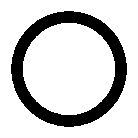
\includegraphics[width=0.02\textwidth]{rond_blanc.pdf}}
\newcommand{\rondBleu}{\protect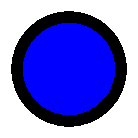
\includegraphics[width=0.02\textwidth]{rond_bleu.pdf}}
\newcommand{\carreBlanc}{\protect
\includegraphics[width=0.02\textwidth]{carre_blanc.pdf}}
\newcommand{\carreBleu}{\protect
\includegraphics[width=0.02\textwidth]{carre_bleu.pdf}}



\title{Construire et exploiter des croyances sur le monde à partir de régularités d'interactions expérimentées}
\author{Florian J. Bernard}
\institute{LIRIS - Université Claude Bernard, Lyon 1\\\email{florian.bernard3@etu.univ-lyon1.fr}}
\date{\today}

\begin{document}
\maketitle
\vfill
% Boucle d'agent
% Dégager l'objet. etre plus haut.
\selectlanguage{francais}
\begin{abstract}
%	Emmanuel Kant définie que la conscience de quelque chose n'est pas réalisée par la chose en soi tel que représenté dans le monde mais par une représentation propre à l'individu. Ce mémoire présente une implémentation de la représentation d'objets à partir d'un agent ayant aucune connaissance sur son environnement.
	
	%Nous nous intéressons à la problématique de la représentation des objets du monde pour le domaine de l'apprentissage développementale (AD). L'AD donne des directions d'implémentations d'un agent n'ayant aucune connaissance de son environnement.
	 Selon Emmanuel Kant, un individu n'a pas accès à la chose en soi tel qu'elle est présente dans le monde, chose que E. Kant appelle noumène, mais construit une représentation interne de cette chose, qu'il appelle phénomène. L'apprentissage développemental donne des directions d'implémentation d'un agent n'ayant pas de connaissances sur son environnement, c'est-à-dire n'ayant pas un accès direct aux noumènes. Il ne possède qu'une liste d'interactions sensorimotrices. Ce mémoire présente une implémentation de la construction de phénomènes à travers le principe de l'apprentissage développemental.
\end{abstract}
\selectlanguage{english}
\begin{abstract}
	According to Immanuel Kant, a person does not known the underlying structure of their world
	"as such" (the noumenal reality), and could only know phenomenal reality (the world "as it appears"
	through their experience). Developmental learning gives some guidelines to implement an agent which has no knowledge on its environment (i.e. does not have access to the noumenal reality). It only use sensorimotor interactions. This paper introduces an implementation of the construction of the phenomenon with the precept of developmental learning.
\end{abstract}

\selectlanguage{francais}
\setcounter{tocdepth}{4}
\tableofcontents
\newpage
%\pagenumbering{arabic}  
\section{Introduction}
% Indicateur visuel sur les mots important la premiere fois qu'ils sont définies

% Contexte générale de la ou je pars, agent congnitif, agnostique. Ensuite
% Expliquer l'apprentissage dével et le modèle.
% Puis le paragraphe
% interactionnisme radical centrale car les interactions. Imposé et le répété tout le temps pour qu'il ne passe pas à côté.
Ce stage se place dans le contexte de l'apprentissage développemental. Ce domaine met en jeu des agents agnostiques (définis section~\ref{par:model_incarne}). Un agent agnostique ne possède pas d'information sur l'environnement dans lequel il évolue et il n'a pas de comportement pré-enregistré. Il possède des méthodes d'apprentissage pour découvrir ses capacités sensorimoteurs en interagissant avec son environnement. L'agent est incarné et développe des mécanismes cognitifs à travers le couplage de son corps physique et l'environnement~\cite{embodied-anderson2003embodied,embodied-brooks1991intelligence}. 

L'apprentissage développemental s'appuie sur le modèle de l'interactionnisme radical qui permet de construire des hiérarchies d'interactions.
% représentés par la figure \reffig{interactions}. 
Ces hiérarchies sont utilisées pour trouver une suite d'interactions permettant de satisfaire l'agent. Le but de cette approche est de construire des comportements augmentant la motivation interactionnelle de l'agent\cite{Liris-5870-interactional-motivation}. 
Néanmoins, l'agent utilisant cette approche ne possède pas de mécanisme lui permettant de représenter les objets du monde.

%\begin{figure}
%\centering
%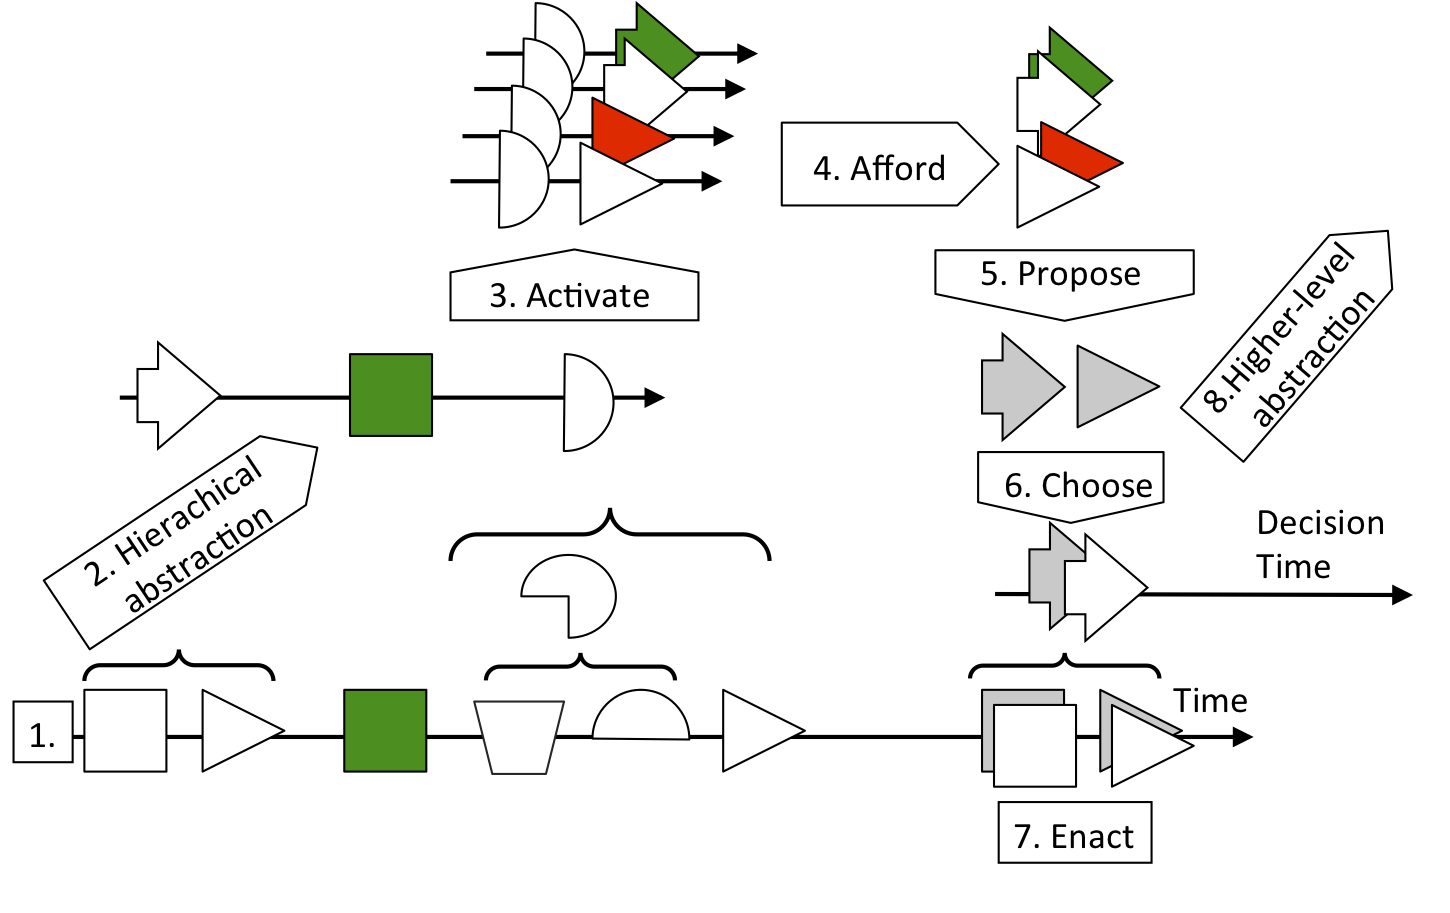
\includegraphics[width=\textwidth]{hierachical_interaction}
%\caption{Apprentissage hiérarchique des interactions}
%\label{fig:interactions}
%\end{figure}
Comment, à partir d'une suite d'interactions ne possédant pas de sémantique, un agent agnostique peut-il construire une représentation des \og~choses~\fg de son environnement~?

La phénoménologie se présente comme l'une des solutions envisageables pour permettre à un agent d'acquérir des connaissances à partir de l'expérience réalisée dans un environnement. La phénoménologie est un courant philosophique qui se concentre sur l'étude des phénomènes, de l'expérience vécue et des contenus de conscience.

% Poser le problème pour que celle ci soit bien introduite.
La phénoménologie a été introduite par Edmund Husserl en 1913. Elle permet, d'un point de vue philosophique, de définir la conscience des choses ainsi~: toute conscience doit être conçue comme conscience de quelque chose. 

\emph{\og~On ne trouve dans la donnée immédiate [de la conscience] rien de ce qui, dans la psychologie traditionnelle, entre en jeu, comme si cela allait de soi, à savoir~: des data-de-couleur, des data-de-son et autres data-de-sensation ~; des data-de-sentiment, des data-de-volonté, etc. Mais on trouve ce que trouvait déjà René Descartes, le cogito, l'intentionnalité, dans les formes familières qui ont reçu, comme tout le réel du monde ambiant, l'empreinte de la langue~: le \og~je vois un arbre, qui est vert~; j'entends le bruissement de ses feuilles, je sens le parfum de ses fleurs, etc.~\fg ~; ou bien \og~je me souviens de l'époque où j'allais à l'école~\fg, \og~je suis inquiet de la maladie de mon ami~\fg, etc. Nous ne trouvons là, en fait de conscience, qu'une conscience de...~\fg} \cite{phenomenologie-husserl}

Selon Emmanuel Kant, pour avoir une conscience de quelque chose, l'individu utilise une représentation interne des \og~choses~\fg du monde qu'on appellera phénomène par la suite. Ces \og~choses~\fg peuvent représenter un objet physique, une relation entre plusieurs objets ou une entité abstraite. A contrario, le noumène désigne la \og~chose~\fg tel qu'elle est dans le monde. Le noumène en lui-même est inaccessible à l'individu qui devra utiliser des phénomènes pour se le représenter. 

Dans ce stage, nous avons réalisé un agent implémentant les 4 principes ci-dessus, à savoir~: 
\begin{itemize}
	\item le concept de l'apprentissage développemental~;
	\item le modèle de l'interactionnisme radical~;
	\item la phénoménologie d'Edmund Husserl~;
	\item la distinction entre les noumènes et les phénomènes.
\end{itemize}

L'agent découvre des régularités de son environnement, à travers ses interactions, et les utilise pour construire des phénomènes. 
Pour visualiser l'état de la mémoire de l'agent, j'ai développé un logiciel gérant la simulation d'agent avec différents algorithmes, un système de visualisation d'interactions et des phénomènes avec la possibilité de tester les agents dans différents environnements. 

La prochaine partie comporte une présentation/état de l'art de l'apprentissage développemental et du modèle de l'interactionnisme radical. La seconde partie explicite la création des phénomènes et des états de croyance. La fin du rapport présente le logiciel de simulation pour finir sur la conclusion.

\subsection{Modèle incarné}
\label{par:model_incarne}
Les propriétés clés du modèle incarné peuvent être résumées par la notion d'inversion du cycle d'interaction illustré en \reffig{inverted_model}~\cite{georgeon2014inverting,varelarosch}, par contraste avec le cycle traditionnel présenté en figure \reffig{traditionnal_model}. 

Un agent conçu avec le modèle incarné est dit \og~agnostique~\fg car il n'a pas de connaissance prédéfinie du monde, et ses données d'entrée (rt) ne représentent pas l'état du monde. Non seulement un agent agnostique n'est pas markovien, mais il n'est pas non plus \og~partiellement markovien~\fg (à la différence des modèles \og~Partially Observable Markov Decision Process~\fg (POMDP)~\cite{Cassandra1994}).

\begin{figure}
	\centering
	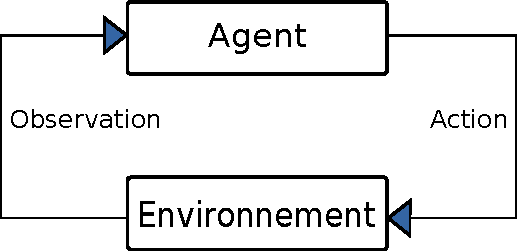
\includegraphics[scale=0.7]{traditionnal_model}
	\caption{Cycle observation/action traditionnel~: les points de début et de fin du cycle ne sont traditionnellement pas explicités. Conceptuellement, le cycle commence par le fait que l'agent reçoit une observation qui est une représentation partielle du monde (possiblement bruitée, symbolique ou non), ensuite, l'agent décide d'une action sur la base de cette observation.}
	\label{fig:traditionnal_model}
\end{figure}

\begin{figure}
	\centering
	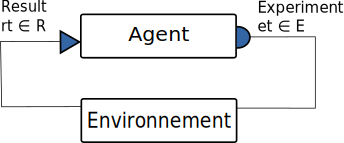
\includegraphics[scale=0.7]{inverted_model}
	\caption{Cycle expérience/Résultat. Le cycle d'interaction commence par le fait que l'agent initie une expérience dans l'environnement (début conceptuel du cycle~: demi-cercle), et se termine par le fait qu'il reçoit un résultat $r_{t}$ de cette expérience (fin conceptuelle du cycle~: triangle). Le résultat $r_{t}$ n'est pas une représentation du monde, car, dans un état du monde donné, l'agent peut recevoir différents résultats en fonction de l'expérience qu'il fait. L'agent doit donc construire sa propre représentation du monde (perception construite) au lieu de la recevoir directement comme c'est le cas dans les modèles traditionnels tels que celui de la figure~\reffig{traditionnal_model}}.
	\label{fig:inverted_model}
\end{figure}

\section{L'Apprentissage Développemental}
L'apprentissage développemental a été, dans un certain sens, introduit par Jean Piaget dans les années 50, lorsqu'il travaillait sur la psychologie développementale~\cite{cognitiviste-piaget1959construction}. En dépit du fait, que les travaux de Piaget ont été menés dans les années 50, l'apprentissage développemental est un nouveau courant de l'intelligence artificiel. Il sollicite des connaissances de plusieurs disciplines comme la robotique, les neurosciences, la psychologie et les sciences cognitives. 
En apprentissage développemental, les agents~:
\begin{itemize}
	\item ne possèdent pas d'ontologie présupposée (i.e~: pas de connaissances présupposées sur le monde)~;
%	\item connaissent que les possibilités d'interactions avec leur environnement~;
%	\item apprennent leurs propres capacités sensorimotrices de façon autonome~;
	\item sont non-markovien, ni même partiellement markovien~;
	\item construisent leur propre représentation de l'environnement qui par définition sera différente de celle que nous pouvons avoir~;
	\item utilisant le concept d'auto-programmation~\footnote{L'auto-programmation est définie comme étant la possibilité de créer un code exécutable qui peut être exécuté au besoin cf.~: \url{http://liris.cnrs.fr/ideal/mooc/lesson.php?n=041}}~\cite{thorisson2013approaches}~;
	\item dispose de possibilités d'interactions sensorimotrices primitives prédéfinies.
\end{itemize}
Le but de l'agent est d'apprendre, découvrir, organiser et exploiter des régularités d'interactions dans le temps et l'espace pour favoriser certains  comportements et améliorer son adaptabilité.

Un point important de l'apprentissage développemental est que l'agent n'est pas un observateur passif de son environnement, il ne réagit pas à un stimuli donné par son environnement, mais choisit volontairement ce qu'il va observer ou réaliser au travers de ses interactions. 
%Pour développer un comportement cognitif, l'agent a besoin d'être incarné dans un corps couplé à un environnement. On parle de l'\emph{embodied paradigm}~\cite{georgeon2014inverting,varelarosch} qui place l'agent comme étant une partie de l'environnement.
% todo
Les interactions sont les éléments centraux de l'agent, elles lui permettent d'interagir avec son environnement et de construire ses connaissances. La modélisation des interactions est un point important pour la conception de l'agent. 

Nous avons choisi d'utiliser le modèle de l'interactionnisme radical qui permet de représenter les actions et les résultats sous forme d'interaction. 

% todo Parler du Embodied Paradigm, du sensorimotor paradigm Constructivist epistemology, Self-programming et après Interactionnisme Radicale de la cognitive architecture.

% Par conséquence la modélisation des interactions est un truc centrale du coup le RI

\subsection{Interactionnisme Radical}
Le modèle de l'interactionnisme radical~\cite{Liris-6480-radical-interactionism} 
%cherche à se rapprocher au mieux des modèles cognitifs de l'apprentissage développemental
est une façon de traduire les idées théoriques de l'apprentissage développemental~\cite{cognitiviste-piaget1959construction,cognitiviste-webster2013mammalian,cognitiviste-o2011red} dans les algorithmes. Dans les modèles cognitifs, l'agent interagit et construit ses connaissances avec son environnement par le biais de ses propres expériences et de leurs résultats. Ce modèle utilise comme primitive les interactions et non le couple expérience/résultat. Les interactions sont développées dans la partie~\ref{par:interaction}

Le modèle est décrit avec la figure \reffig{model_radical_interactionnism}.
% todo mieux détailler et expliquer en fonction du papier d'olivier.
À l'initialisation, l'agent possède une liste prédéfinie d'interactions sensorimotrices \emph{I}, appelées \textbf{interactions primitives}. À chaque cycle de décisions, l'agent choisit une interaction appelée \textbf{interaction intended} qu'il tentera de réaliser dans l'environnement. L'interaction effectivement réalisée dans l'environnement, appelée \textbf{interaction enacted} est retournée à l'agent. Les interactions \intended et \enacted appartiennent à la même liste d'interactions sensorimotrices \emph{I}. 

Il est à noter que l'agent ne connaît pas les conséquences des différentes interactions ni sur l'environnement ni sur lui-même et des liens qui peuvent exister entre chaque interaction. De plus, nous ne souhaitons donner aucune heuristique qui pourrait l'aider à comprendre ces interactions.

L'environnement représente le couplage entre le corps de l'agent et le monde. %Le corps ne comprend que des expériences et retourne un résultat fonction de la réussite de l'expérience. L'exécution permet de transformer une interaction en expérience que le corps puisse mettre à exécution puis reconstruit les interactions en fonction des résultats retournés par le corps. 
Les mécanismes mis en place dans le système décisionnel permettent~:
% La \emph{décision} permet de sélectionner une interaction, appelé \intended en fonction des précédentes interactions réalisées. L'\emph{action} décortique cette interaction et la réalise à travers le corps de l'agent dans l'environnement. Comme l'\intended est une suggestion, celle-ci peut échouer et une autre interaction peut-être réalisée à la place de celle-ci. Une fois l'interaction réalisé dans l'environnement, l'action renvoie l'interaction résultat, appelée \enacted, à la décision qui pourra alors sélectionner la prochaine interaction à réaliser. Les mécanismes misent en place dans la décision permettent~:
\begin{itemize}
	\item d'apprendre des interactions sur plusieurs niveaux 
	%comme dans la figure \reffig{interactions}
	 tout en évitant l'explosion combinatoire~;
	\item de sélectionner la prochaine interaction en fonction du contexte d'interaction précédemment réalisée. 
\end{itemize}

\begin{figure}
	\centering
	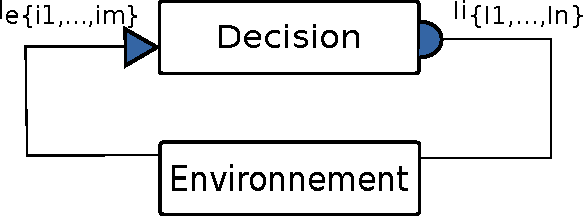
\includegraphics[scale=0.7]{model_radical_interactionnism}
	\caption{Modèle de l'interactionnisme radical}
	\label{fig:model_radical_interactionnism}
\end{figure}
L'agent étant agnostique~\cite{Liris-5510-environment-agnostic}, c'est-à-dire, qu'il ne connaît pas du tout l'environnement, il interagit avec celui-ci uniquement aux travers des interactions qu'il possède. L'agent découvre des suites d'interactions qui sont avantageuses de son point de vue. 
%Pour \emph{avancer}, l'agent apprend les mécanismes intéressants qui lui permettront de trouver des suites d'interactions lui permettant de réaliser les interactions avantageuses. 


Le système de décision ne commence pas par une observation donnée par l'environnement 
%comme dans la figure \ref{fig:model_standard} 
mais par une interaction sélectionnée par l'agent. 
L'agent est donc pro-actif, il sélectionne la prochaine interaction qu'il souhaite \enact en prenant en compte l'expérience passée de l'agent et non une fonction de l'environnement.

%L'agent est alors maître des observations/actions qu'il réalise dans l'environnement et les mécanismes mises en place se concentre uniquement sur la sélection de la prochaine interaction en prenant en compte l'expérience de l'agent et non une fonction de l'environnement. 

%\begin{figure}
%	\centering
%	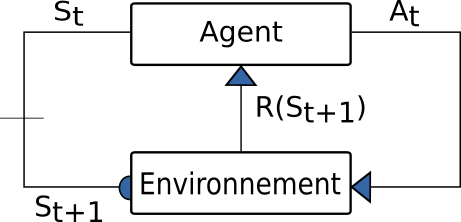
\includegraphics[scale=0.7]{model_standard}
%	\caption{Modèle d'un agent avec l'apprentissage par renforcement}
%	\label{fig:model_standard}
%\end{figure}
% \todo Étoffer le qlearning

\subsection{Interaction} \label{par:interaction}
Dans le contexte des interactions,
%Une interaction part du principe que l'
on ne peut pas dissocier une perception d'une action. Elle est composée d'un couple abstrait action/résultat défini \textit{a priori} qui est indépendant de l'environnement, du système sensoriel et des actionneurs que possède l'agent. Elle n'a pas de sémantique et ne définit pas un état du monde. Les interactions caractérisent le \emph{couplage} entre l'agent et l'environnement. Les algorithmes mis en place dans le système décisionnel doivent prendre en compte le fait que la connaissance de l'agent se construit uniquement à travers les interactions.

Pour que l'agent puisse apprendre et exploiter ses connaissances, l'algorithme de décision permet d'apprendre des interactions composites sur plusieurs niveaux. Celles-ci donnent à l'agent la possibilité de développer des comportements de plus haut niveau.

Une \textbf{interaction composite} est composée d'une pré-interaction et d'une post-interaction (qui elles mêmes peuvent-être composites ou primitives). La pré-interaction renseigne sur le contexte dans lequel l'agent se trouve. La figure \reffig{decision_learn_and_selection} indique le processus d'apprentissage et de sélection des interactions composites.

%TODO refaire le graphic
\begin{figure}
	\centering
	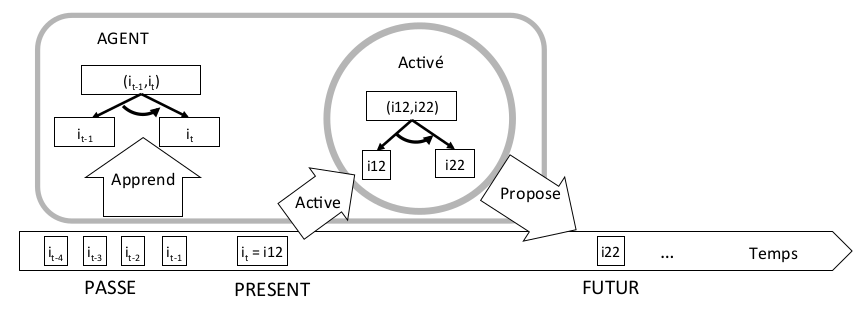
\includegraphics[scale=0.35]{principle_learn_and_selection_decision}
	\caption{Principe d'apprentissage et de sélection d'une interaction composite. Afin de déterminer la prochaine interaction, la décision sélectionne toutes les interactions composites ayant comme pré-interaction l'interaction précédemment \enacted \{i12\}. Puis, analyse l'interaction composite qui a le plus de chance d'être \enact avec la plus forte motivation interactionnelle. L'interaction composite ainsi sélectionnée a comme pré-interaction l'interaction \enacted \{i12\} et comme post-interaction l'interaction à réaliser.
		}
	\label{fig:decision_learn_and_selection}
\end{figure}

Pour pouvoir réaliser cet apprentissage, l'agent doit pouvoir~:
\begin{itemize}
	\item décomposer une interaction composite \intend~;
	\item reconstruire une interaction composite \enact.
\end{itemize}

Une interaction composite est exécutée en une seule fois. Elle peut réussir ou échouer sur chaque interaction primitive qu'elle possède.

%Une interaction composite est une interaction qui ne possède pas d'action et de résultat, mais une pré-interaction et une post-interaction. Elle permet à l'agent d'interagir de manière plus élaboré avec son environnement en fonction du contexte que chaque interaction composite met en place implicitement. 

\begin{figure}
	\centering
	
\includegraphics[scale=0.13]{interactions_composites_string_problem}
	\caption{Interactions \intended (ligne 1) et \enacted (ligne 2) d'un flux d'interaction.}
	\label{fig:interactions_composites_string_problem}
\end{figure}
La figure \reffig{interactions_composites_string_problem} est une sous partie d'un flux d'interactions réalisées par un agent utilisant les interactions composites.
La première interaction a été correctement prévu par l'agent. À l'inverse la deuxième a échoué car l'interaction \intended \{\carreBleu\} est différente de l'interaction \enacted \{\carreBlanc\}. L'interaction composite \intended \{\triangleBlanc, \carreBleu\} a échoué sur la post-interaction \{\carreBlanc\}. 
% L'interaction composite intended a échoué et l'interaction enacted est \{\carreBlanc\}. 

Une \textbf{interaction alternative} est une interaction qui peut-être \enact à la place d'une interaction \intended. Dans la figure \reffig{interactions_composites_string_problem}, l'interaction \{\carreBlanc\} est une interaction alternative à l'interaction \{\carreBleu, \rondBlanc, \carreBlanc, \triangleBlanc\}. Cette propriété n'est pas symétrique.
% par exemple, l'interaction \{\carreBlanc, \triangleBlance\} n'est pas une interaction alternative de l'interaction \{\carreBleu\}.

Lorsque l'alternative est symétrique, c'est-à-dire que deux interactions sont alternatives l'une de l'autre alors on parle d'\textbf{interaction opposée} et de \textbf{régularité immédiate}. Les interactions \{\carreBlanc\} et \{\carreBleu\} sont des interactions opposées l'une à l'autre.

%L'agent connaît les résultats possibles pour chaque action qu'il peut réaliser car l'apprentissage développementale définie qu'un résultat n'est pas une fonction de l'environnement, mais bien une perception interne à l'agent. L'agent connaît donc toutes les interactions qu'il peut réaliser dans l'environnement, mais ne connais pas leurs significations et ne sait pas a priori celle qu'il peut faire. 
% Par exemple, l'agent possède l'interaction manger/OK et manger/KO. Lors de la simulation il peut ne jamais croiser d'objet pouvant être manger. Alors il réalisera uniquement manger/KO et l'interaction manger/OK ne sera jamais utiliser. Par conséquence, il ne pourra pas déterminer si cette interaction est réalisable et comment réussir à la réaliser. L'agent se crée alors une perception active de son environnement. \cite{SIMON}


Afin que l'agent puisse sélectionner une interaction plutôt qu'une autre, une motivation permet de les différencier. %les interactions reposent sur une motivation qui permet de les différencier les unes aux autres.
\subsection{Motivation}

Pour que l'agent puisse déterminer les interactions intéressantes, le concept de motivation interactionnelle~\cite{Liris-5870-interactional-motivation} est mis en place dans l'apprentissage développemental. Ce concept permet de définir des interactions \emph{plaisantes} et \emph{déplaisantes} pour l'agent. Grâce à cette motivation l'agent sélectionne une interaction sans autre but que la satisfaction qu'elle peut lui procurer~\cite{cognitiviste-interactionnel-steels2004autotelic}. Elle est implémentée grâce à une valence définie \textit{a priori}. Si la valence est positive (resp. négative), l'interaction est plaisante (resp. déplaisante). Si la valence est nulle, l'interaction en elle même n'apporte rien à l'agent, par contre couplée avec d'autres interactions, celle-ci peut amener aux interactions plaisantes. 

D'autres formes de motivations sont également prises en compte et permettent de construire des comportements différents~:
\begin{itemize}
	\item l'agent aime prévoir les prochaines interactions à \enact~;
	\item l'agent peut être \og~curieux~\fg~: l'agent va préférer tester les liens entre les différentes interactions pour avoir le plus de choix possibles, et potentiellement avoir la meilleure approche~;
	\item l'agent peut être \og~joueur~\fg~: l'agent va répéter des interactions dans le but de les réutiliser par la suite dans un autre contexte. 
\end{itemize}
% Il peut être "curieux"~: 
% Il peut être "joueur"~:
%Ces motivations sont propre à l'agent et lui permette d'être plus ou moins curieux impliquant un apprentissage différents des suites d'interactions possibles dans divers contextes d'interaction. Il peut aussi être joueur et répéter des interactions pour leur permettre d'avoir un poids plus important que d'autre. Ces comportements lui permettent d'organiser les interactions en fonction de ce que l'agent apprécie.

% Perspective 

% Premier algorithme permettant de séparé l'action de la décision avec la décomposition des interactions composites.


%Les algorithmes \refalg{agent_action}, \refalg{decompose_interaction_action} et \refalg{recompose_interaction_action} explicite la partie action de l'agent. 
%
%\begin{algorithm}[H]
%	
%	\SetAlgoLined
%	\DontPrintSemicolon
%	\SetKwFunction{FGetPrimitiveInteraction}{getPrimitiveInteraction}
%	\SetKwProg{Func}{Function}{}{}
%	Interaction $\leftarrow$ "NULL"\;
%	CurrentInteraction $\leftarrow$ "NULL"\;
%	\Func{\FGetIntend{}}
%	{
%		\If {CurrentInteraction $=$ "NULL"} {
%			Interaction $\leftarrow$ decision.getIntend() \;
%			createExperiencesSequence() \;
%		}
%	}
%}
%\KwRet CurrentInteraction\;
%}
%\caption{Action~: récupération de l'interaction à effectuer dans l'environnement}
%\label{alg:agent_action}
%\end{algorithm}
%
%\begin{algorithm}[H]
%		\SetAlgoLined
%		\DontPrintSemicolon
%		\SetKwFunction{FGetPrimitiveInteraction}{getPrimitiveInteraction}
%		\SetKwProg{Func}{Function}{}{}
%		Interaction $\leftarrow$ "NULL"\;
%		CurrentInteraction $\leftarrow$ "NULL"\;
%		\Func{\FGetIntend{}}
%		{
%			\If {CurrentInteraction $=$ "NULL"} {
%				Interaction $\leftarrow$ decision.getIntend() \;
%				createExperiencesSequence() \;
%			}
%		}
%	}
%	\KwRet CurrentInteraction\;
%}
%\caption{Action~: récupération de l'interaction à effectuer dans l'environnement}
%\label{alg:agent_action}
%\end{algorithm}

\subsection{Modèle de programmation d'un agent}
\begin{figure}
	\centering
	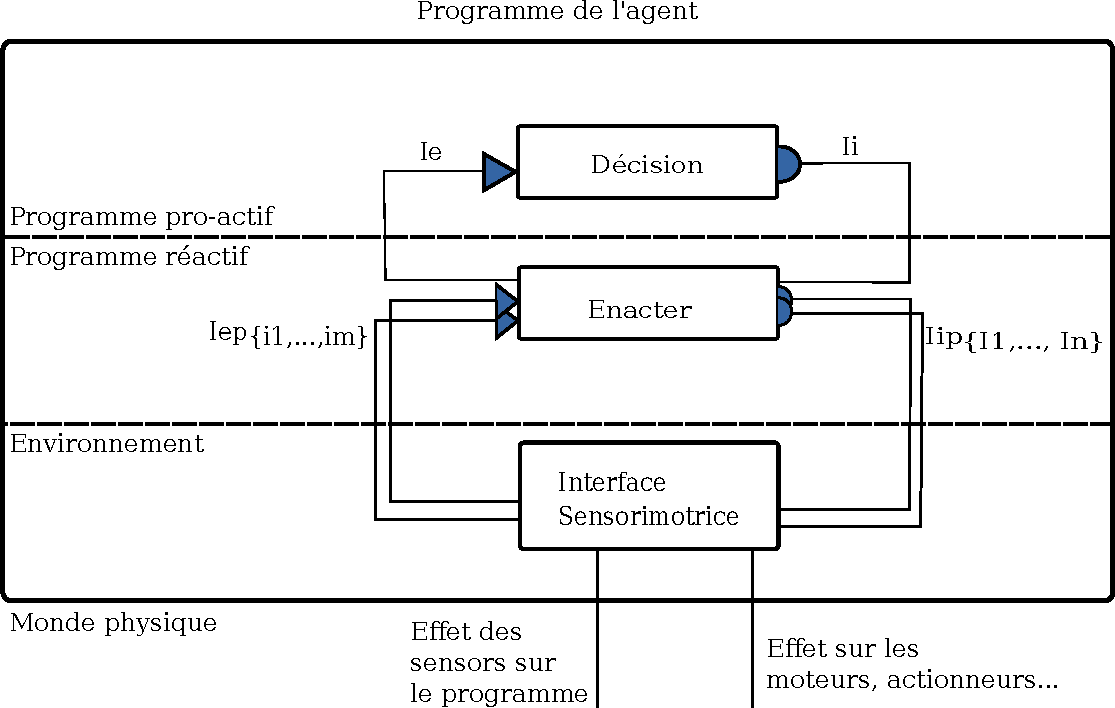
\includegraphics[scale=0.6]{program_model}
	\caption{Schéma de l'implémentation d'un agent}
	\label{fig:prog_model}
\end{figure}
La figure \reffig{prog_model} explicite l'implémentation d'un agent avec le modèle de l'interactionnisme radical. La partie pro-active possède les mécanismes d'apprentissage et de sélection des interactions. Elle sélectionne une interaction (primitive ou composite) \emph{Ii} qui sera réalisé à l'aide de la partie réactive. L'\emph{enacter} décompose, si besoin, l'interaction \intended \emph{Ii} en interaction primitive \emph{Iip$_1$}…\emph{Iip$_n$}et l'exécute à travers les différentes interfaces sensorimotrices. Les résultats des capteurs se présentent sous la forme d'interactions primitives \enacted \emph{Iep$_1$}…\emph{Iep$_m$}. La taille de l'interaction composite \enacted peut être inférieure ou égale à la taille de l'interaction \intended. L'\emph{enacter} reconstruit l'interaction composite \enacted \emph{Ie} et la retourne à la décision qui va pouvoir apprendre de nouvelles interactions. Dans la suite du mémoire, la partie pro-active de l'agent sera mise en avant. Nous considérons que le programme réactif et l'environnement sont fonctionnels. 

\subsection{L'espace}
Mes travaux se basent sur la thèse de Simon Gay~\cite{Liris-7032-simon-thesis} et sur le MOOC réalisé par Olivier Georgeon\footnote{\url{http://liris.cnrs.fr/ideal/mooc/}}. Tous deux ont travaillés sur le modèle de l'interactionnisme radical. S. Gay s'est orienté sur la représentation de l'espace et des objets que l'environnement permet d'afforder~\cite{affordance-gibson}. \og~Une affordance est définie comme une possibilité d'interaction proposée par l'environnement à un agent. En effet, dans ces expériences, chaque objet révèle qu'il peut être saisi par un certain mouvement, et, de ce fait, afforde ce mouvement.~\fg. Durant sa thèse, S. Gay a grandement travaillé sur la représentation de l'espace dans un agent implémentant l'apprentissage développemental et la perception d'objet dans l'espace observable et de l'espace global. 

La représentation des objets est réalisée avec la \emph{signature d'interaction}. Une signature d'interaction est représentée par un ensemble d'interactions dont le succès caractérise la présence ou l'absence d'un objet affordé par les interactions. Si des interactions possèdent les mêmes signatures alors celles-ci relatent du même objet. 

Les mécanismes de décision se servent de ces signatures pour effectuer les interactions satisfaisantes. 

Son travail a été une source d'inspiration pour la réalisation de ce stage. La représentation des \emph{objets} du monde met en place une partie des mécanismes associés aux signatures.

\section{Énoncé du problème}
Le problème est défini en se mettant à la place de l'agent (n.b.~: L'environnement est présenté de manière plus conventionnelle au paragraphe~\ref{par:string_problem}). Nous ne connaissons rien de l'environnement et nous devons créer une structure permettant de représenter les connaissances construites par l'agent. 
% de définir les différents \emph{objets} du monde.
 Les interactions de la figure \reffig{interactions_string_problem} représentent les perceptions et les actions de l'agent. 
À partir du flux d'interactions de la figure \reffig{interactions_flux_hedonism_string_problem}, nous souhaitons que l'agent découvre des régularités qu'il puisse exploiter. 
% Sous section je pose le problème avec les graphique flux et interaction et finis par la suite va montrer une méthode permettant de résoudre ce problème.

% Présenter Ou je suis et ma contribution.


% Tout de suite se mettre en abstraction
% Développer la base pour montrer la dissociation entre l'agent et l'environnement.
\begin{figure}
	\centering
	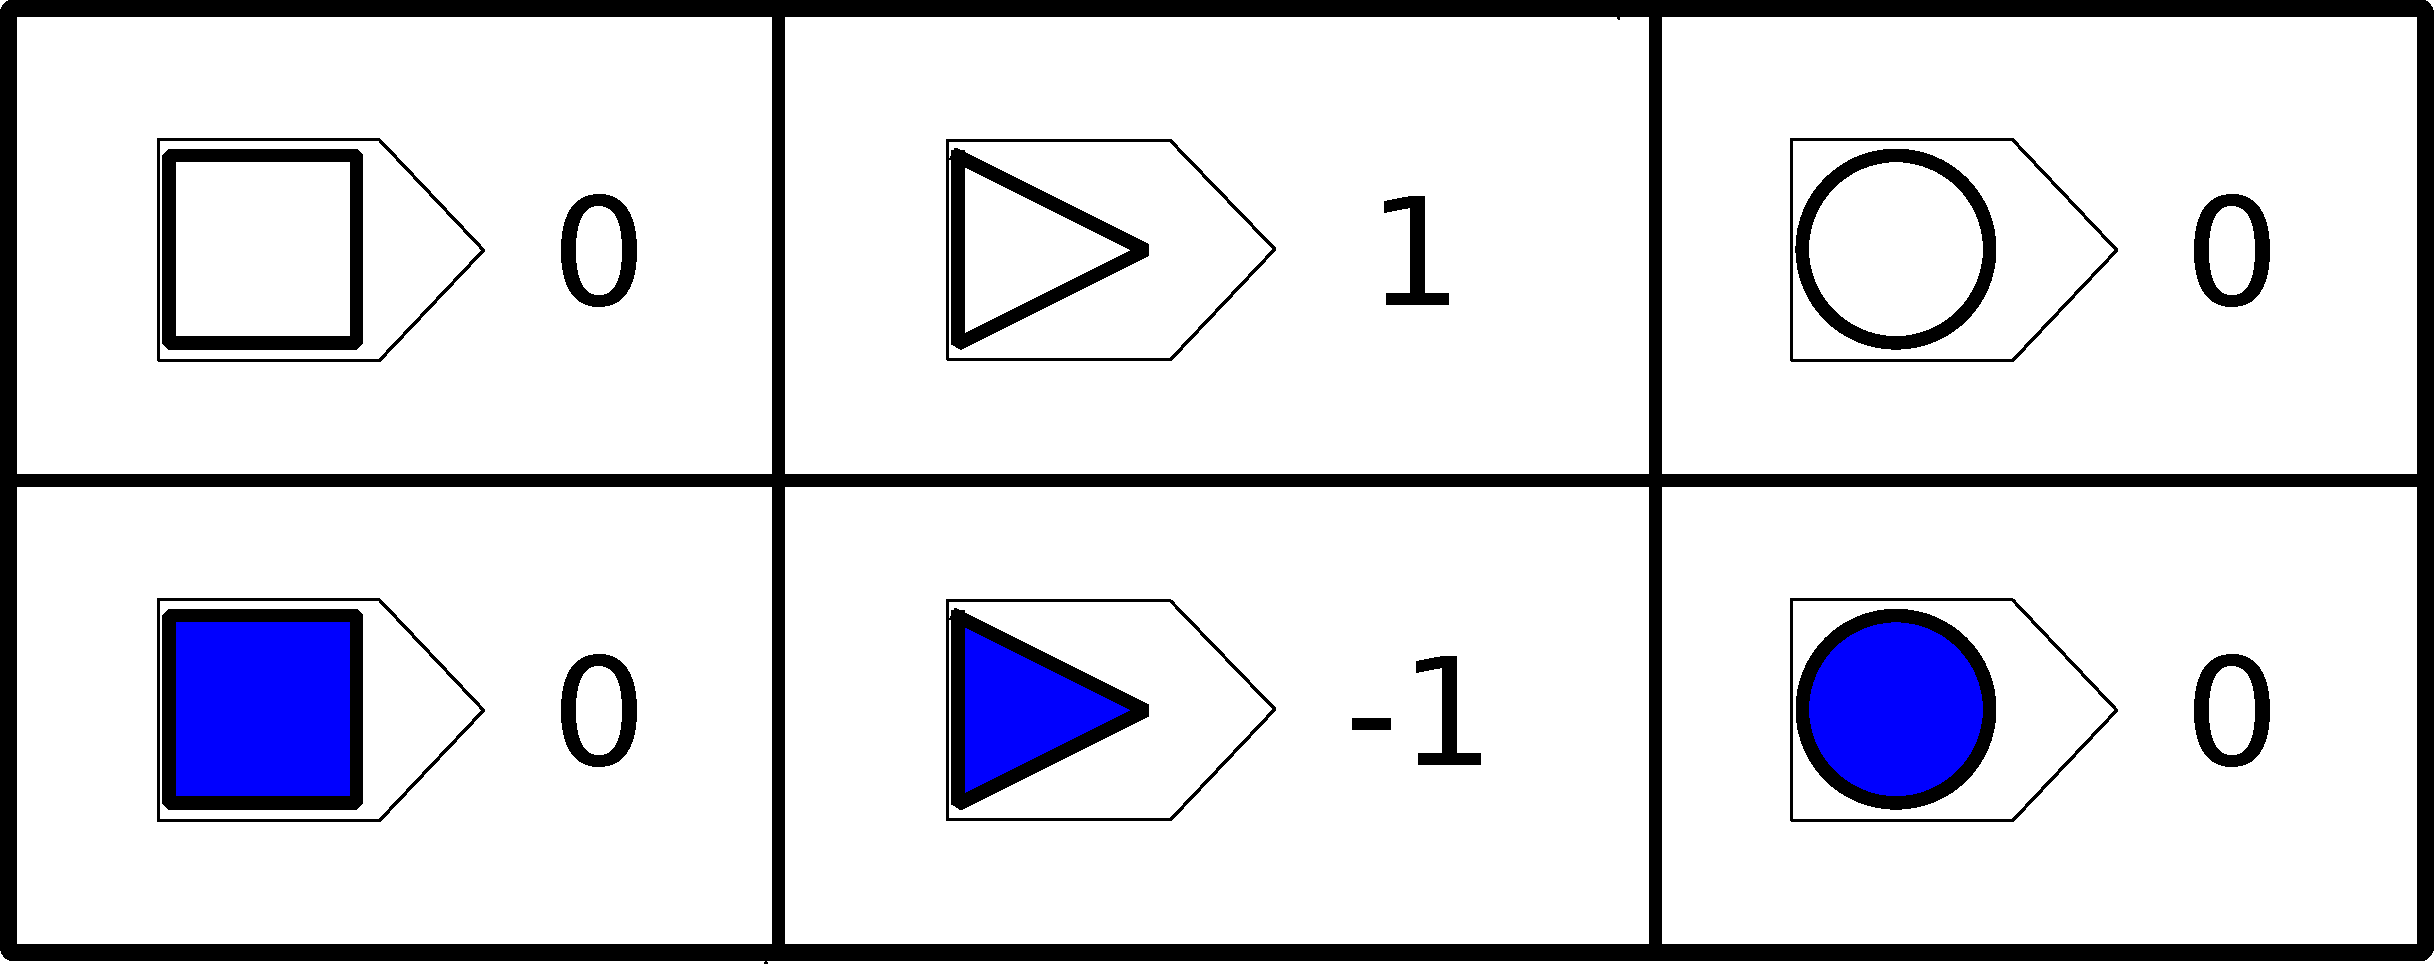
\includegraphics[scale=0.1]{interactions_string_problem}
	\caption{Liste des interactions que possède l'agent dans l'environnement inconnu. }
	\label{fig:interactions_string_problem}	
\end{figure}

\begin{figure}
	\centering
	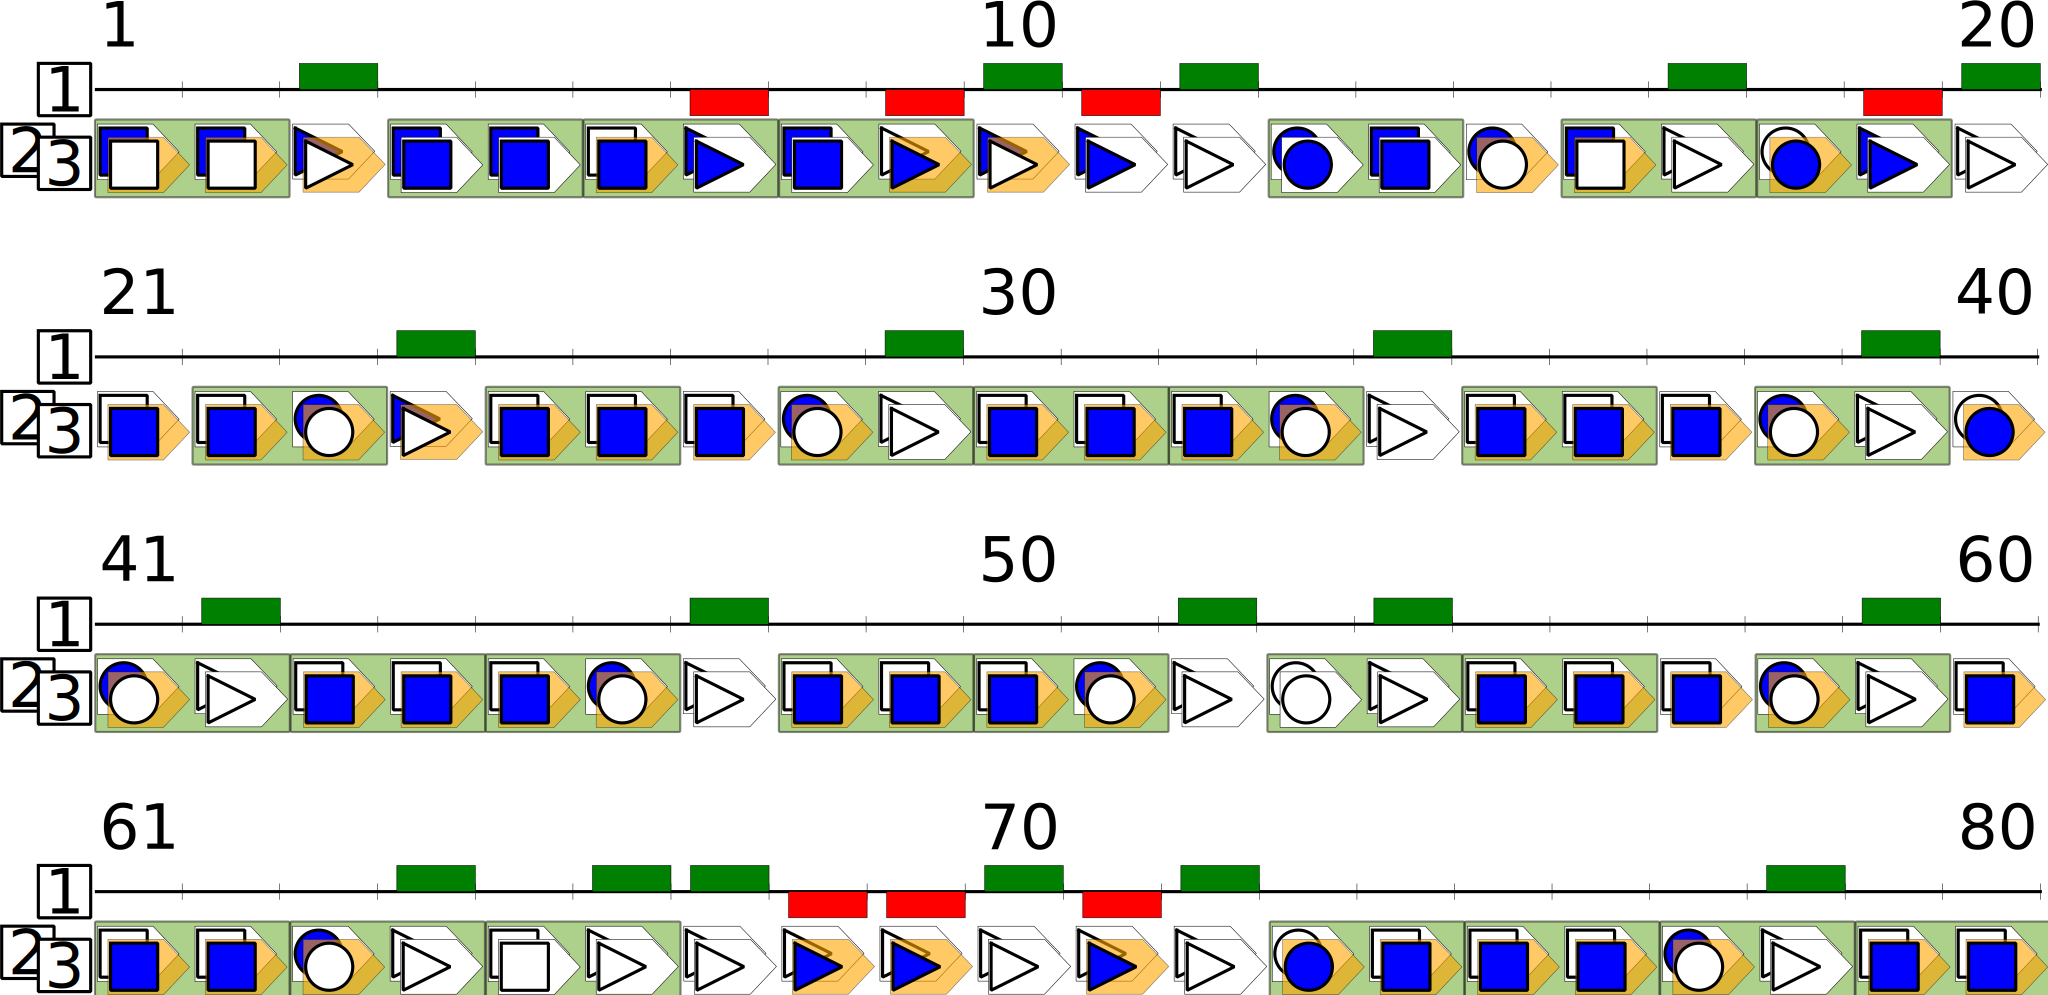
\includegraphics[scale=0.08]{flux_interactions_hedonism_string}
	\caption{Flux d'interactions réalisé par l'algorithme d'O. Georgeon disponible sur le MOOC\protect\footnotemark. La ligne \num{1} représente la valence qui caractérise la motivation interactionnelle. En vert, la valence est positive, l'interaction est plaisante. En rouge l'interaction est déplaisante, la valence est négative. L'absence de symbole indique que l'interaction n'apporte rien. La ligne \num{2} est l'interaction \intended et la ligne \num{3} est l'\enacted. Les interactions en orange ont été mal prévues par l'agent qui est alors insatisfait. L'agent a bien prédit les interactions \enacted blanche par conséquence son humeur est satisfaite.}
	\label{fig:interactions_flux_hedonism_string_problem}
\end{figure}
\footnotetext{\url{http://liris.cnrs.fr/ideal/mooc/lesson.php?n=058}}
À partir du flux d'interactions de la figure \reffig{interactions_flux_hedonism_string_problem} nous pouvons trouver~:
\begin{itemize}
	\item les régularités immédiates~;
	\item des régularités séquentielles~;
\end{itemize}

Les régularités immédiates sont données grâce aux lignes \num{2 et 3}. Au début du flux d'interaction, l'agent \intend des interactions sans savoir si elles sont réalisables. Régulièrement, l'interaction \enacted ne correspond pas, ce qui implique que cette interaction est une interaction alternative. Au pas 1, l'interaction \{\carreBleu\} a pour alternative \{carre blanc\}. Au pas 6, les interactions \{\carreBleu\} et \{\carreBlanc\} deviennent des interactions opposées l'une à l'autre.

Les régularités séquentielles de niveau 2 que l'on peut trouver via ce flux sont représentées par la figure \reffig{regularities_string_problem}. Ces régularités sont définies par l'environnement, et nous posons l'hypothèse qu'avec ces régularités, l'agent peut construire des connaissances sur l'environnement. 

La régularité d'interactions \{\carreBlanc\}, \{\carreBlanc\} informe sur la présence d'une observation. Cette interaction est supposée répétable indéfiniment. Elle est considérée comme étant une \textbf{interaction persistante} qui renseigne sur la présence ou l'absence d'un objet. Les interactions \{\rondBleu\}, \{\triangleBlanc\} et \{\triangleBleu\} ne se répètent pas de manière systématique, on considère que ce sont des interactions qui modifient l'environnement et sont appelées \textbf{interactions sporadiques}. L'interaction \{\rondBlanc\} ne donne pas d'informations particulières sur son état, par contre elle renseigne des interactions qui peuvent être effectuées juste après elle.

\begin{figure}
	\centering
	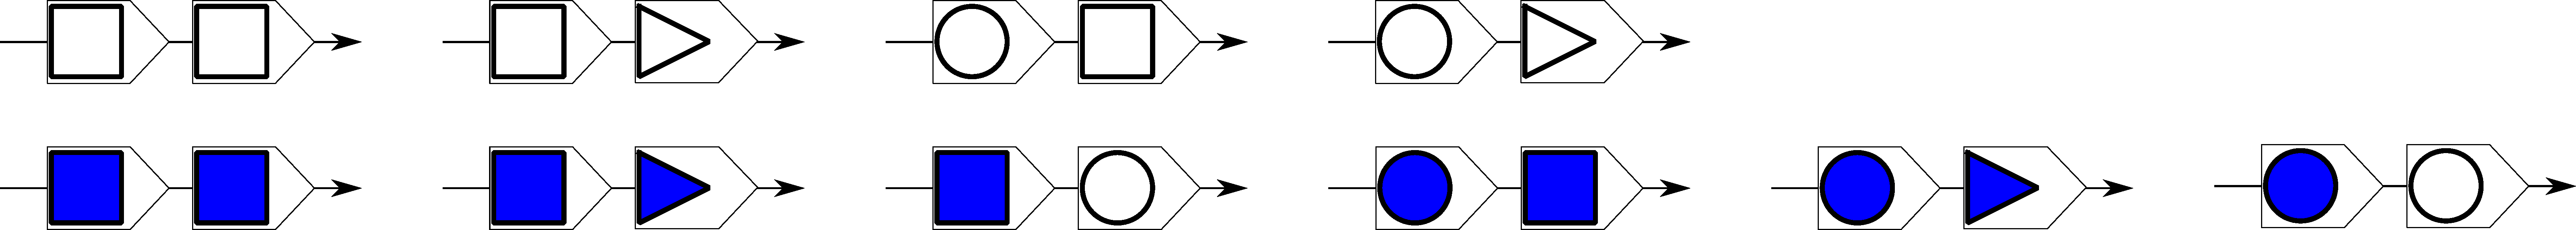
\includegraphics[scale=0.08]{regularities_string_problem}
	\caption{Régularités observées dans le flux d'interaction. Ces régularités sont tirées du flux d'interaction de la figure~\reffig{interactions_flux_hedonism_string_problem}. Elles sont liées aux interactions \enacted. Par exemple, la régularité \num{3} est réalisée au pas 15.}
	\label{fig:regularities_string_problem}	
\end{figure}

L'agent est motivé par la réalisation de l'interaction \{\triangleBlanc\}, de ce fait, nous espérons pouvoir construire les régularités séquentielles de la figure \reffig{well_regularities_string_problem}. Ces régularités sont déjà apprises par l'algorithme via les interactions composites mais ces interactions ne permettent pas d'avoir une représentation des \emph{objets} de l'environnement. 

\begin{figure}
	\centering
	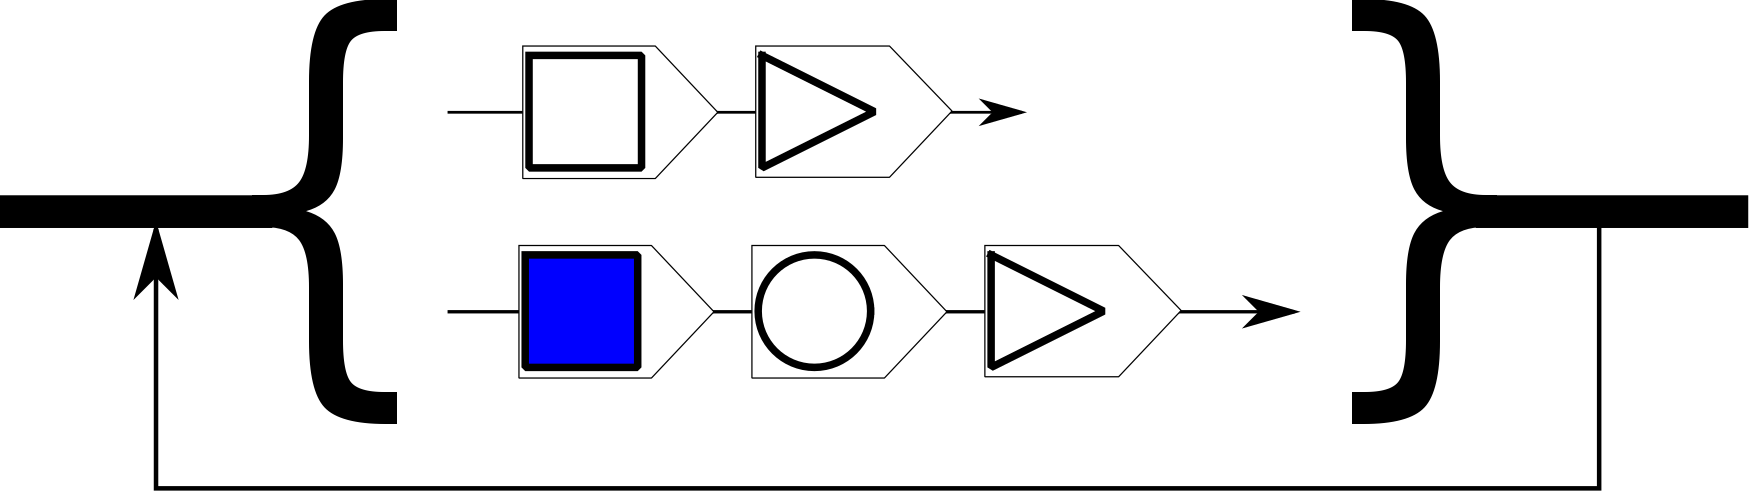
\includegraphics[scale=0.1]{well_regularities_string_problem}
	\caption{Régularités séquentielles que l'on souhaiterait que l'agent trouve et utilise pour satisfaire sa motivation}
	\label{fig:well_regularities_string_problem}
\end{figure}

Les interactions sporadiques \{\rondBlanc\} et \{\rondBleu\} permettent une fois \enacted de réaliser respectivement les interactions persistantes \{\carreBlanc\} et \{\carreBleu\}. Nous appelons \textbf{état de croyance} l'information qui permet à une interaction sporadique de prédire une interaction persistante. L'interaction \{\carreBlanc\} permet d'\enact l'interaction \{\triangleBlanc\}. L'interaction \{\rondBlanc\} permet de changer l'environnement de sorte que l'interaction persistante \{\carreBlanc\} soit toujours \enact. De ce fait, l'interaction \{\rondBlanc\} possède comme état de croyance l'interaction persistante \{\carreBlanc\}. 

Avec ces informations et en considérant que l'interaction \{\rondBlanc\} est par défaut une interaction sporadique, nous pouvons créer le graphe de Pétri de la figure \reffig{petri_hedonism_string_problem} qui représente les liens entre les interactions persistantes et sporadiques. 
%TODO À refaire !!! Etoffer le graphe de Petri à refaire
\begin{figure}
	\centering
	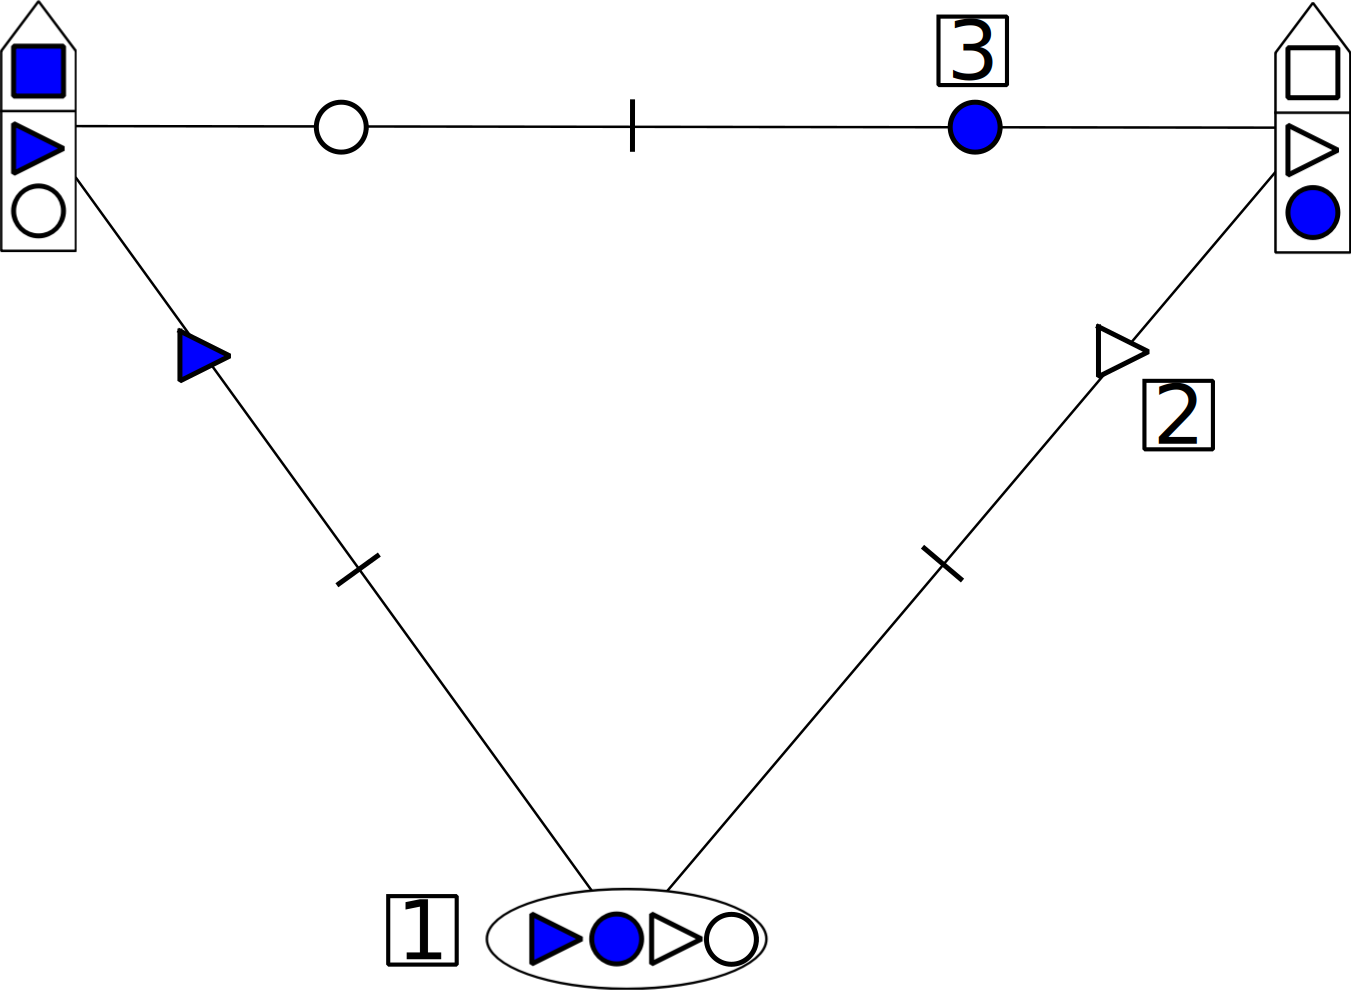
\includegraphics[scale=0.1]{petri_hedonism_string_problem}
	\caption{Graphe de Pétri que nous souhaitons que l'agent construise par rapport aux régularités de niveau 2 de la figure~\reffig{regularities_string_problem}. Le nœud~\num{1} représente l'état de croyance \emph{unknown} qui regroupe les interactions sporadiques. Les autres nœuds représentent les interactions considérées comme persistantes. La partie inférieure des nœud représente les interactions qui pourront être réalisées lorsque l'agent se trouve dans cet état de croyance. Lorsque l'agent est dans l'état de croyance <\carreBlanc> et qu'il réalise l'interaction \{\triangleBlanc\} alors l'état de croyance deviendra \emph{unknown}. Ce lien est représenté par le \num{2}. Le \num{3} représente un état de croyance associé à l'interaction sporadique \{\rondBleu\}. }
	\label{fig:petri_hedonism_string_problem}
\end{figure}

%Lors des expérimentations, un agent possédant des interactions comme dans la figure \reffig{interactions_string_problem} crée le flux d'interaction de la figure \reffig{interactions_flux_string_problem}, qui retrace son activité au sein d'un environnement. L'agent arrive à interagir avec son environnement tout en maximisant sa motivation intrinsèque. Par contre, il ne construit pas de connaissance lui permettant d'appréhender les objets du monde. Je propose par la suite, une structure et des méthodes permettant à un agent de construire une représentation des objets du monde, tout en maximisant sa motivation intrinsèque.

%\begin{figure}
%	\centering
%	
\includegraphics[scale=0.05]{whole_interactions_flux_minimum_algo_string_problem}
%	\caption{Flux d'interactions effectué par l'agent dans l'environnement inconnu. La ligne \num{1} représente la valeur de la motivation interactionnelle de l'interaction, en vert la valence est positive, en rouge négative et nulle sur la ligne. La ligne \num{2} est l'interaction intended et la ligne \num{3} est l'enacted. Les interactions en jaune ont été mal prévu par l'agent qui est alors insatisfait. La ligne \num{4} représente l'état de croyance dans lequel l'agent est. La ligne \num{5} symbolise l'humeur de l'agent. Du pas 1 à 5, l'agent est de plus en plus excité car l'interaction qu'il effectue peut se répéter. À l'étape 6, il crée le phénomène \{\carreBlanc\}, sont état d'excitation retombe à zéro et il devient curieux car la tables d'usage de l'interaction \{\carreBlanc\} est vide. La ligne \num{6} permet de visualiser la création/modification des phénomènes et des états de croyance. Les interactions persistantes sont représentés par un rectangle avec un triangle et les états de croyance des interactions sporadiques par un rectangle.}
%	\label{fig:interactions_flux_string_problem}
%\end{figure}

%Nous faisons l'hypothèse que l'agent peut construire des connaissances sur son environnement uniquement en utilisant les interactions.
%Pour ce faire, nous posons la question de comment à partir d'une suite d'interaction, cf. figure \reffig{interactions_flux_string_problem}, un agent peut tirer des régularités d'interactions. La figure \reffig{regularities_string_problem} montre les régularités d'interaction que l'environnement, dans lequel évolue l'agent, propose. Comme pour l'agent, nous ne connaissons pas cette suite d'interactions, leur signification et les liens entre-elles.  
%

%\cite{phenomenologie}.


%Intuitivement, nous observons que..
%Nous pouvons, d'un point de vue extérieur à l'agent, constater que les interactions de mêmes formes sont des interactions opposées et que les interactions \emph{carrés} renseigne sur un objet distinct. L'agent, quant-à lui, doit trouvé ces régularités immédiates afin de comprendre que certaines interactions sont possibles dans un contexte et non l'expérience en elle-même. Puis trouver les régularités séquentielles, cf. figure \reffig{well_regularities_string_problem}qui lui permettront de satisfaire sa motivation intrinsèque.
\subsubsection{Environnement du \emph{string problem}}
\label{par:string_problem}
L'environnement décrit avec les \emph{yeux} de l'agent est le \emph{string problem}~\cite{Liris-6368-string-problem}. Cet environnement est une chaîne de nombres~: 1-7-3-2-9-3-5-6-7-8-1-2-4-0-9-8-5-4-6-0, que l'agent doit trier. L'agent est positionné sur un nombre et peut~:
\begin{itemize}
	\item avancer vers un nombre plus grand (resp. plus petit) avec l'interaction \{\carreBlanc\} (resp. \{\carreBleu\})~;
	\item échanger le nombre sur lequel il se situe avec celui devant lui. Si après l'échange le nombre devant est plus grand (resp. plus petit) alors l'interaction \{\rondBlanc\} (resp. \{\rondBleu\}) est \enact~;
	\item avancer sur un nombre plus grand (resp. plus petit) via l'interaction \{\triangleBlanc\} (resp. \{\triangleBleu\}).
\end{itemize} 
%L'interaction \{\carreBlanc\} (respectivement \{\carreBleu\}) indique que le prochain nombre est supérieur (resp. inférieur) à celui ou l'agent se trouve. L'interaction \{rond X\} permet à l'agent d'intervertir deux nombres. Si après la conversion, le nombre devant l'agent est plus petit (resp. plus grand) alors l'interaction enacté sera  \{\rondBlanc\} (reps. \{\rondBleu\}). L'agent avance sur un nombre plus grand avec l'interaction \{\triangleBlanc\} et sur un nombre plus petit avec \{\triangleBleu\}. 
%\todo{Attention à l'interpretation de l'agent avec la phrase suivante on pense que l'agent connaît l'environnement.}
De notre point de vue, l'agent est motivé à trier la chaîne de caractères pour, par la suite, réaliser l'interaction \{\triangleBlanc\}. Pour lui, la chaîne de caractères n'existe pas et pour le moment évolue dans un environnement qui donne du plaisir lors de l'\emph{énaction} de l'interaction \{\triangleBlanc\}.
Cet environnement est volontairement simple pour rendre accessible l'analyse de la mémoire de l'agent.

De ces constats, je propose une structure permettant à l'agent d'obtenir une représentation des objets à travers ses interactions primitives.
% À partir de ce constat, je vais par la suite répondre à la question~: Quel est la structure basée les interactions permet de créer une représentation d'un objet~?

\section{Les phénomènes et les tables d'usage}
\subsection{Tables d'usages}
Les tables d'usage sont inspirées du travail que S. Gay a réalisé lors de sa thèse et qu'il appelle \emph{signature}. Chaque interaction primitive possède une tables d'usage. Elles sont définies par la figure~\reffig{usage_table_white_circle_string_problem}.% se rapproche. 

\begin{figure}
	\centering
	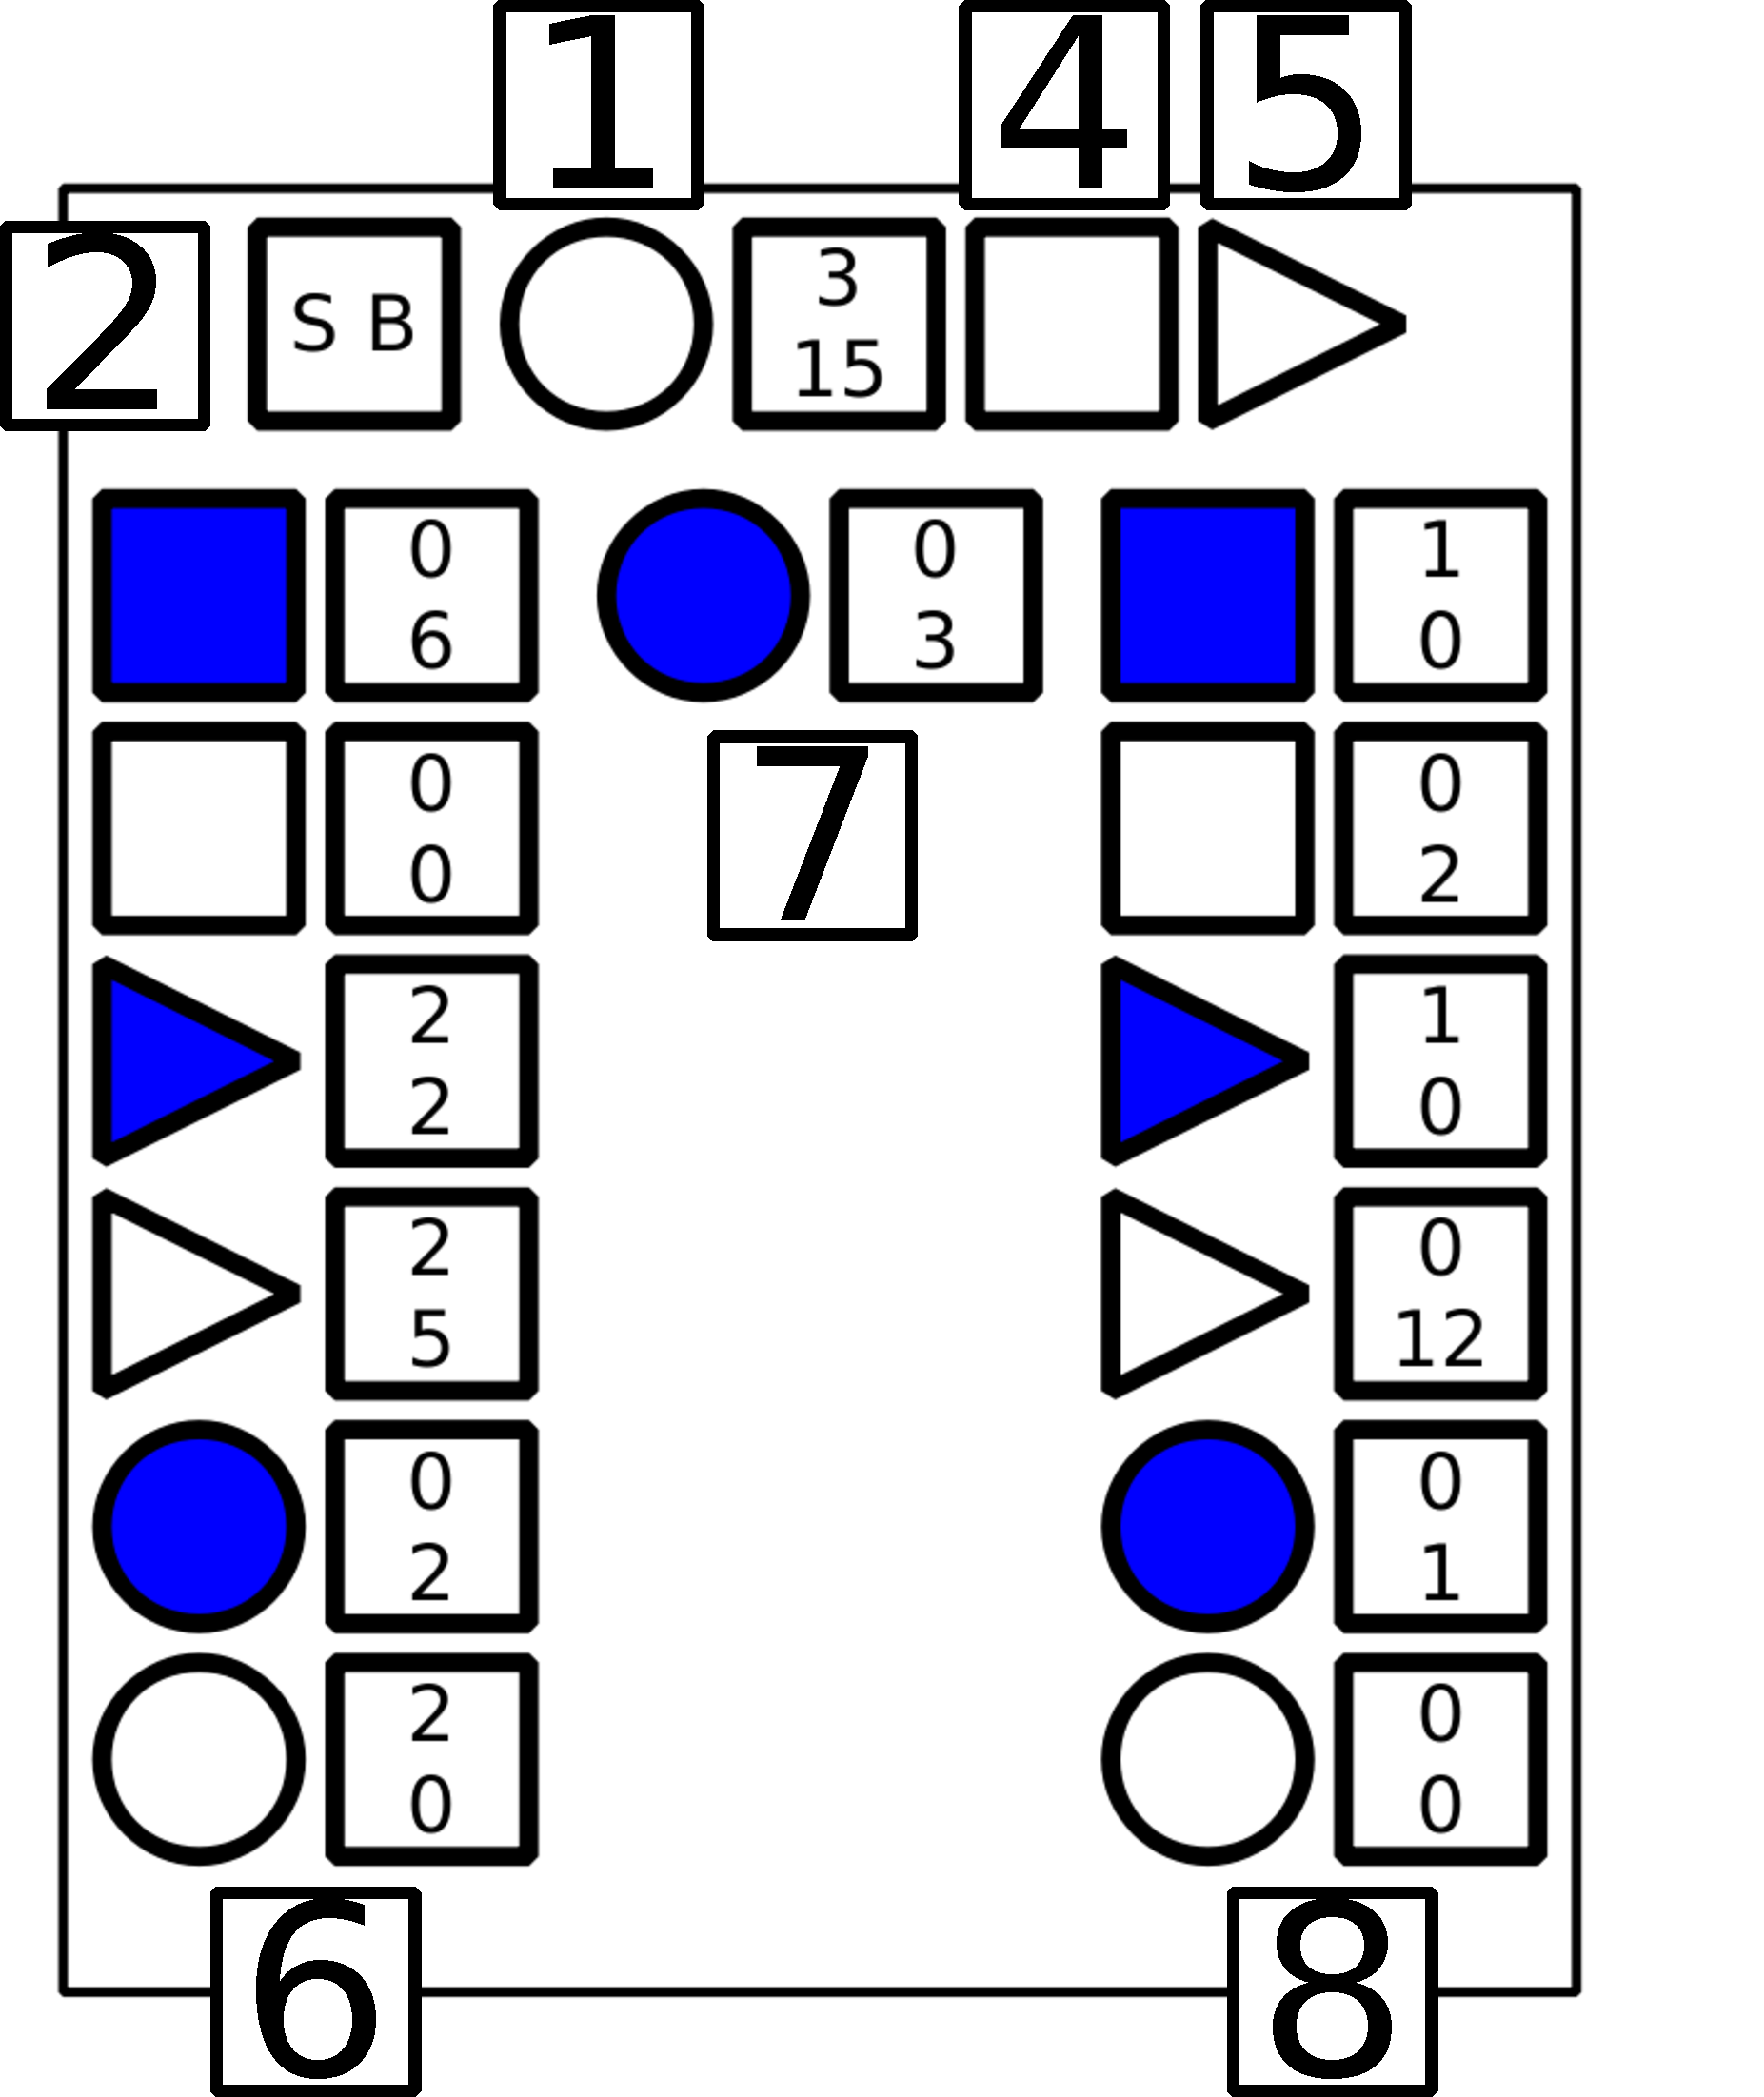
\includegraphics[scale=0.2]{usage_table_white_circle_string_problem}
	\caption[forlist]{%forlist
		Table d'usage de l'interaction \{\rondBlanc\} représenté par le \num{1}. Le \num{2} est le type de l'interaction qui peut-être~: \begin{inparaenum}
				\item P~: interaction persistante~;
				\item S~: interaction sporadique~;
				\item S~B~: interaction sporadique avec un état de croyance (i.e.~: Sporadic with Believe).
				\end{inparaenum}
			Les cases avec les nombres représentent le nombre de fois que l'interaction à gauche a été \intended (en haut) et \enacted (en bas). Le \num{4} est l'état de croyance de l'interaction. Le \num{5} est la prochaine interaction qui sera \intended si l'agent \enact cette interaction, elle est retrouvée grâce à une simulation de la décision. La colonne \num{6} liste les pré-interaction, la \num{7} les interactions opposées et la \num{8} les post-interactions}
	\label{fig:usage_table_white_circle_string_problem}
\end{figure}

Une récompense est associée par chaque tables d'usage qui correspond pour une interaction~:
\begin{itemize}
	\item persistante~: à la valence de la meilleur interaction confirmé~;
	\item sporadique~: à la valence de l'interaction~;
	\item sporadique avec croyance~: à la valence de l'interaction plus la moitié de l'état de croyance.
\end{itemize}

%Les tables d'usages sont utilisées pour représenter les liens entre les différentes interactions. Une tables d'usage maintient à jour le nombre de fois que l'interaction a été intended et enacted dans les différents contexte d'interaction. Pour se faire, les tables d'usage possède une liste de~:
%\begin{itemize}
%	\item pré-interaction~;
%	\item post-interaction~;
%	\item interaction alternative/opposée.
%\end{itemize}
%
%La figure \reffig{usage_table_blue_circle_string_problem} montre l'interaction sporadique \rondBleu et sa tables d'usage.

%Une tables d'usage comporte une liste des pré-interactions primitives et une autre pour les post-interactions primitives. En plus, elle possède une valeur de récompense qui associe la valence de l'interaction à celle que la tables d'usage permet d'\enact.

%Le \num{2} est l'interaction de la tables d'usage. Les carrés contenant deux chiffre représente le nombre de fois a été intended et enacted. Le \num{4} est l'interaction attachée à l'état de croyance (pour une interaction persistente, l'état de croyance est l'interaction en elle-même). Le num{5} est la future interaction qui sera réalisé lorsque l'agent aura enacted l'interaction. 
%Le \num{6} représente les pré-interactions. 
%Le \num{7} liste les interactions alternative et le \num{8} sont les post-interactions.

On peut déduire de la tables d'usage de la figure \reffig{usage_table_white_circle_string_problem} que l'interaction \{\rondBlanc\} n'est pas répétable car la table des pré-interactions indique qu'elle a été \intended 2 fois, mais jamais \enacted. 
L'interaction \{\carreBlanc\} n'est pas réalisable avant l'interaction \{\rondBlanc\} car celle-ci a été \intended 2 fois sans jamais être \enacted. 

Toujours avec la table des pré-interactions, les interactions \{\carreBleu\} et \{\rondBleu\} ont toujours été \enacted avec succès, ce sont donc des interactions qui permettent d'\enact l'interaction \{\rondBlanc\}. Elles sont les conditions qui permettent d'\enact de manière \emph{certaine} (i.e. du point de vue de l'agent) l'interaction \{\rondBlanc\}.

De la même manière avec la table des post-interactions, l'interaction \{\rondBlanc\} permet d'\enact \{\carreBlanc\}, \{\rondBleu\} et \{\triangleBlanc\}. Elles sont appelées d'interactions confirmées par l'interaction \{\rondBlanc\}. 

L'interaction \{\rondBleu\} est une interaction opposée et qui a été \enacted trois fois à la place de l'interaction \{\rondBlanc\}.

Avec cette interaction nous pouvons construire le sous graphe de Pétri de la figure \reffig{sub_petri_white_circle} qui reprend les points ci-dessus.
%TODO finir la figure de Petri
\begin{figure}
	\centering
	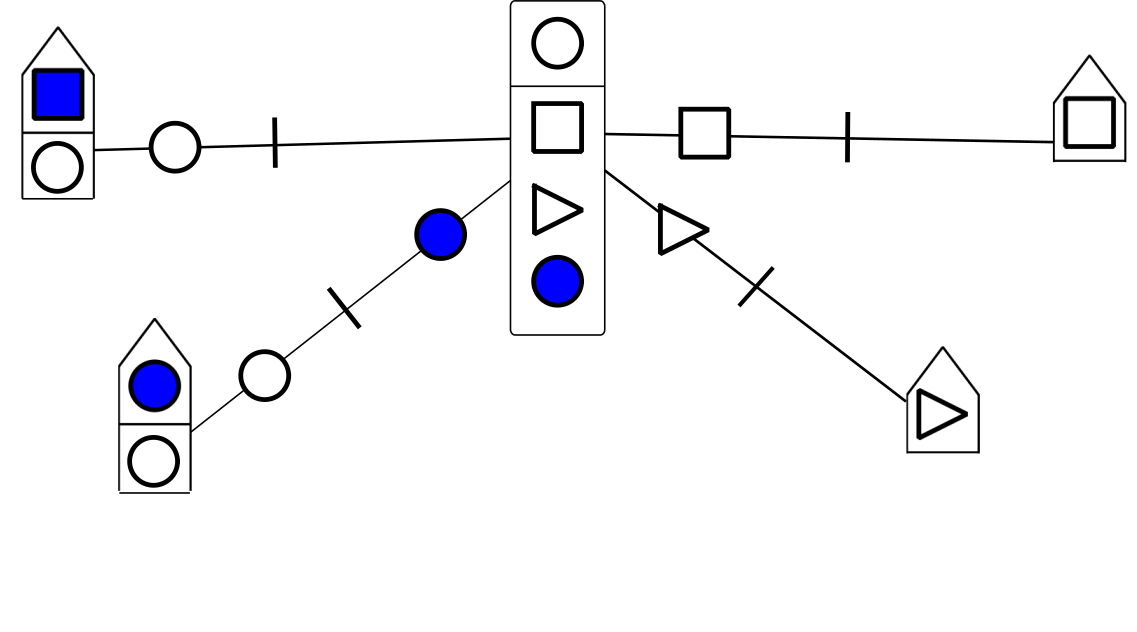
\includegraphics[scale=0.2]{sub_petri_white_circle}
	\caption{Sous graphe de Petri de l'interaction \{\rondBlanc\} dans le contexte de figure~\reffig{usage_table_white_circle_string_problem}}
	\label{fig:sub_petri_white_circle}
\end{figure}
% Chaqeu interaction a sa tables d'usage qui lui permttent de maintenir les liens et avec les autres interactions et donc de représenter des info de contexte.
%La tables d'usage permet de maintenir un lien avec les différentes interactions et met en place une sorte de contexte d'un niveau pour chaque interaction. 

%Les tables d'usage sont mise à jour lors de la phase d'\emph{enacter} de la figure~\reffig{prog_model} et sont utilisées lors de la phase de décision pour le choix de l'interaction suivante.

\subsubsection{Mise à jour des tables d'usages}
Lorsque l'\emph{enacter}~(cf. \reffig{prog_model}) à réaliser l'interaction \intended et a recréé l'interaction \enacted, il met à jour les tables d'usages des deux interactions à travers la structure appelée \emph{Phénomènes}. 

La mise à jour est effectuée en utilisant le principe suivant~:
\begin{itemize}
	\item l'interaction \enacted doit mettre à jour les poids de succès ou de l'échec des pré-interactions \intended et \enacted~;
	\item l'interaction précédemment \enacted met à jour les poids de succès ou d'échec des post-interactions \intended et \enacted~;
	\item Si l'interaction \intended est différente de l'interaction \enacted alors l'interaction \intended doit mettre à jour le poids d'échec de la précédente interaction \enacted~;
	\item Si l'interaction \intended est égale à la précédente interaction \intended mais que les interactions \enacted sont différentes alors l'interaction \intended est considérée comme sporadique.
\end{itemize}

\subsubsection{Table d'usage pour les interactions composites}
Pour le moment, les interactions composites sont gérées de la même manière que les interactions primitives mais n'apportent pas d'information pertinente dans la représentation des objets de l'environnement. Par conséquence, elles ne seront pas détaillées dans ce mémoire.

\subsection{Phénomènes}
\emph{Nota~bene}~: dans le domaine de la phénoménologie, les objets du monde se représentent non pas par l'objet en lui-même mais par les interactions que l'individu peut effectuer sur l'objet. Les composantes du monde sont inaccessibles à l'individu, mais celui-ci arrive à distinguer les objets \emph{rond} et \emph{carré} facilement. Le fait de voir un objet active dans le cerveau une sorte de simulation des interactions que nous pouvons effectuer avec l'objet. Cette représentation nous donne la possibilité de comprendre que deux objets sont identiques dans des situations différentes~\cite{singe-murata1997object}. Pour permettre la gestion des phénomènes, nous avons implémenté 2 algorithmes. 
\subsubsection{Système décisionnel \num{1}}
Ce système décisionnel possède deux phases. L'une pour l'apprentissage des phénomènes et la seconde pour l'exploitation et la mise à jour des connaissances. Les interactions sont initialisées comme étant inconnues. L'agent va répéter, jusqu'à un certain seuil, une interaction considérée comme inconnue, pour déterminer si elle est persistante ou sporadique. Le flux d'interactions généré par cet algorithme dans le \emph{string problem} est représenté par la figure \reffig{flux_interactions_minimum_algorithm_string_problem}. 

\begin{algorithm}[h]
	
	\SetAlgoLined
	\DontPrintSemicolon
	\SetKwFunction{FGetIntend}{getIntend}
	\SetKwProg{Func}{Function}{}{}
	Believe $\leftarrow$ "unknown"\;
	mood $\leftarrow$ "curious"\;
	\Func{\FGetIntend{}}
	{
		\eIf {mood $=$ "curious"} {
			intended $\leftarrow$ leastTriedExperiment(Believe) \;
		}{
		\eIf{mood $=$ "hedonist"} {
			intended $\leftarrow$ intendedMaxExpectedOutcomeValence(Believe)\;
		} {
		\If{mood $=$ "excited"} {
			intended $\leftarrow$ lastEnacted\;
		}
	}
}
\KwRet intended\;
}
\caption{Algorithme de sélection de l'interaction \intended}
\label{alg:minimum_algorithm_intended}
\end{algorithm}
%
L'algorithme \refalg{minimum_algorithm_intended} sélectionne une interaction \intended. Les différentes humeurs permettent à l'algorithme de différencier l'apprentissage de l'exploitation. L'humeur \emph{excited} est utilisée pour reproduire la précédente interaction \intended afin de déterminer si cette interaction est persistante ou sporadique. Elle sera déterminée dans l'algorithme \refalg{minimum_algorithm_enacted}. L'humeur \emph{curious} favorise, dans le contexte de l'interaction \enacted, la réalisation de test sur les post-interactions les moins utilisées. L'\emph{hedonist} est le comportement par défaut. Il sélectionne l'interaction qui à le plus de chance d'être \enacted et qui privilégie la motivation interactionnelle. La sélection de cette interaction est détaillé dans l'algorithme \refalg{maxExpectedOutcomeValence}

L'algorithme \refalg{minimum_algorithm_enacted} permet de sélectionner l'humeur de l'agent en fonction de l'interaction \enacted. Si l'agent était excité, alors il compare la précédente interaction \enacted avec la nouvelle~:
\begin{itemize}
	\item si les interactions sont identiques et que le seuil d'excitation n'est pas atteint alors l'agent est toujours excité par cette interaction~;
	\item si les interactions sont identiques et que le seuil d'excitation est atteint alors l'interaction est considérée comme persistante~;
	\item si les interactions sont différentes alors l'interaction \enacted est sporadique.
\end{itemize}
Ensuite l'agent met à jour son état de croyance développé par la fonction \emph{updateAndGetBelieve}. Après, si l'interaction \enacted est inconnue, alors l'agent va être excité et va donc répéter cette interaction pour déterminer si elle persistante ou sporadique. Si la table des post-interactions comporte des interactions non testées dans le contexte de l'interaction \enacted, alors l'agent va être curieux et expérimenter une interaction jamais \intend et \enact. Sinon il devient hédoniste.

La fonction \emph{updateAndGetBelieve} permet de mettre à jour l'état de croyance de l'interaction \enact. Si elle est persistante, alors l'état de croyance sera l'interaction elle-même. Si l'interaction sporadique possède une post-interaction perstante et qui est confirmé, alors l'état de croyance sera la post-interaction persistante, sinon il sera inconnu. 

L'algorithme~\refalg{maxExpectedOutcomeValence} sélectionne l'interaction la plus intéressante dans le contexte de l'état de croyance courant~:
\begin{itemize}
	\item si l'état de croyance existe~: sélectionne une interaction satisfaisante ou une interaction amenant a une interaction satisfaisante~;
	\item l'ineteraction est sporadique~: retourne une interaction persistante qui a le plus de chance d'être \enact.
\end{itemize}

%
\begin{algorithm}[h]
	\SetAlgoLined
	\DontPrintSemicolon
	\SetKwFunction{FHasEnacted}{hasEnacted}
	\SetKwProg{Proc}{Procedure}{}{}
	\Proc{\FHasEnacted{Interaction enacted}}
	{
		\If {mood $=$ "excited"} {
			\eIf{enacted $\ne$ lastEnacted} {
				enacted.setUnpersistent()\;
			} {
			\eIf{excitement $>$ excitementThreshold} {
				enacted.setPersistent()\;
			} {
			excitement ++\;
		}
	}
}
Believe $\leftarrow$ updateAndGetBelieve(intended, enacted)\;
\If {mood $\ne$ excited} {
	mood $\leftarrow$ "hedonist"\;
} 
\eIf {enacted.isUnknown()} {
	mood $\leftarrow$ "excited"\;
	lastEnacted $\leftarrow$ enacted\;
} {
\If {all the experiments have not been tried yet in the context of believe} {
	mood $\leftarrow$ "curious"\;
}
}
\KwRet\;
}
\caption{Mise à jour de la décision lors de la réalisation d'une interaction}
\label{alg:minimum_algorithm_enacted}
\end{algorithm}

\begin{algorithm}[h]
	\SetAlgoLined
	\DontPrintSemicolon
	\SetKwFunction{FIntendedMaxExpectedOutcomeValence}{intendedMaxExpectedOutcomeValence}
	\SetKwProg{Func}{Function}{}{}
	\Func{\FIntendedMaxExpectedOutcomeValence{UsageTable believe}} {
		\eIf{believe $!=$ NULL} {
			\ForEach{interactionList $e$ of believe.getPostInteraction()}{
				\If{$e$.isConfirm()} {
					addAnticipation($e$.getInteraction()\;
					\Indp , $e$.getReward()\;
					, $e$.getFactor()\;
					)\;
				}
			}
		} {
		\ForEach{interactionList $e$ of lastEnacted.getPostInteraction()}{
			\If{$e$.isPhenomena()}{
				addAnticipation($e$.getInteraction()\;
				\Indp , $e$.getReward()\;
				, $e$.getFactor()\;
			}
		}
	}
\KwRet bestInteractionInAnticipation()\;
}
\caption{Algorithme de sélection de la meilleur interaction.}
\label{alg:maxExpectedOutcomeValence}
\end{algorithm}

\begin{figure}
	\centering
	\includegraphics[scale=0.08]{0-80_flux_interactions_minimum_algorithm_string_problem}
	\caption{Flux d'interaction de l'algorithme d'apprentissage et d'exploitation. La ligne \num{4} représente l'état de croyance dans lequel se trouve l'interaction \enacted. En gris, l'état de croyance est inconnue, en blanche elle fais référence a l'état de croyance <\carreBlanc> et en bleu à l'état de croyance <\carreBleu>. 
		La ligne \num{6} montre la création et la mise à jour des interactions perstantes et sporadique. 		
		L'humeur de l'agent est sur la ligne \num{5}. Du pas 1 à 6, l'excitation de l'agent augmente jusqu'au seuil (prédéfini). Au pas 7, l'interaction \{\carreBlanc\} est considérée comme persistante. Au pas 8, l'agent est curieux car il connaît l'interaction persistante \{\carreBlanc\}, mais sa tables d'usage est vide. Il va alors essayer une expérience\protect\footnotemark~qui permettra de remplir une partie de la tables d'usage. Au pas 9, l'agent est excité par l'interaction \enacted \{\triangleBlanc\}, mais au pas 10, cette interaction n'est pas répétée. Elle est alors considérée comme étant une interaction sporadique. De même pour l'interaction \{\triangleBleu\} du pas 10 au 12. Au pas 18, l'agent a créé les deux phénomènes attendus à savoir <\carreBlanc> et <\carreBleu>. Mais ces phénomènes sont incomplets. Avec les différents tests, l'agent remplira correctement la tables d'usage des phénomènes <\carreBlanc> et <\carreBleu> au pas 27. L'exploitation commence, avec des erreurs au pas 32. À partir de ce moment, l'agent se sert de ses croyances pour avancer, mais celui-ci se trompe encore car les tables d'usages ne sont pas correctement remplies. Ce n'est qu'à partir du pas 49 que les différents liens sont correctement établis et que l'exploitation peut se dérouler sans erreur.}
	\label{fig:flux_interactions_minimum_algorithm_string_problem}
\end{figure}
%TODO d'enactage...
\footnotetext{Une expérience correspond au test d'énactage d'une interaction ou de l'une de ses opposées.}

\newpage

\subsubsection{Système décisionnel \num{2}}
Le second algorithme % part du principe que l'apprentissage des interactions sporadiques peut être réalisé en même temps que l'exploitation. L'agent va apprendre de ses erreurs et essayer de maximiser sa motivation interactionnelle.
% Les interactions sont initialisées comme étant
initialise les interactions comme étant
 persistantes et l'agent va alors apprendre au cours de son expérience les interactions sporadiques. La figure \reffig{flux_interactions_phenomena_string_problem} relate l'expérience de l'agent avec cet algorithme dans l'environnement du \emph{string problem}. La figure \reffig{evole_petri_phenomenology_string_problem} montre l'évolution des états de croyance de l'agent.

\begin{figure}
		\centering
		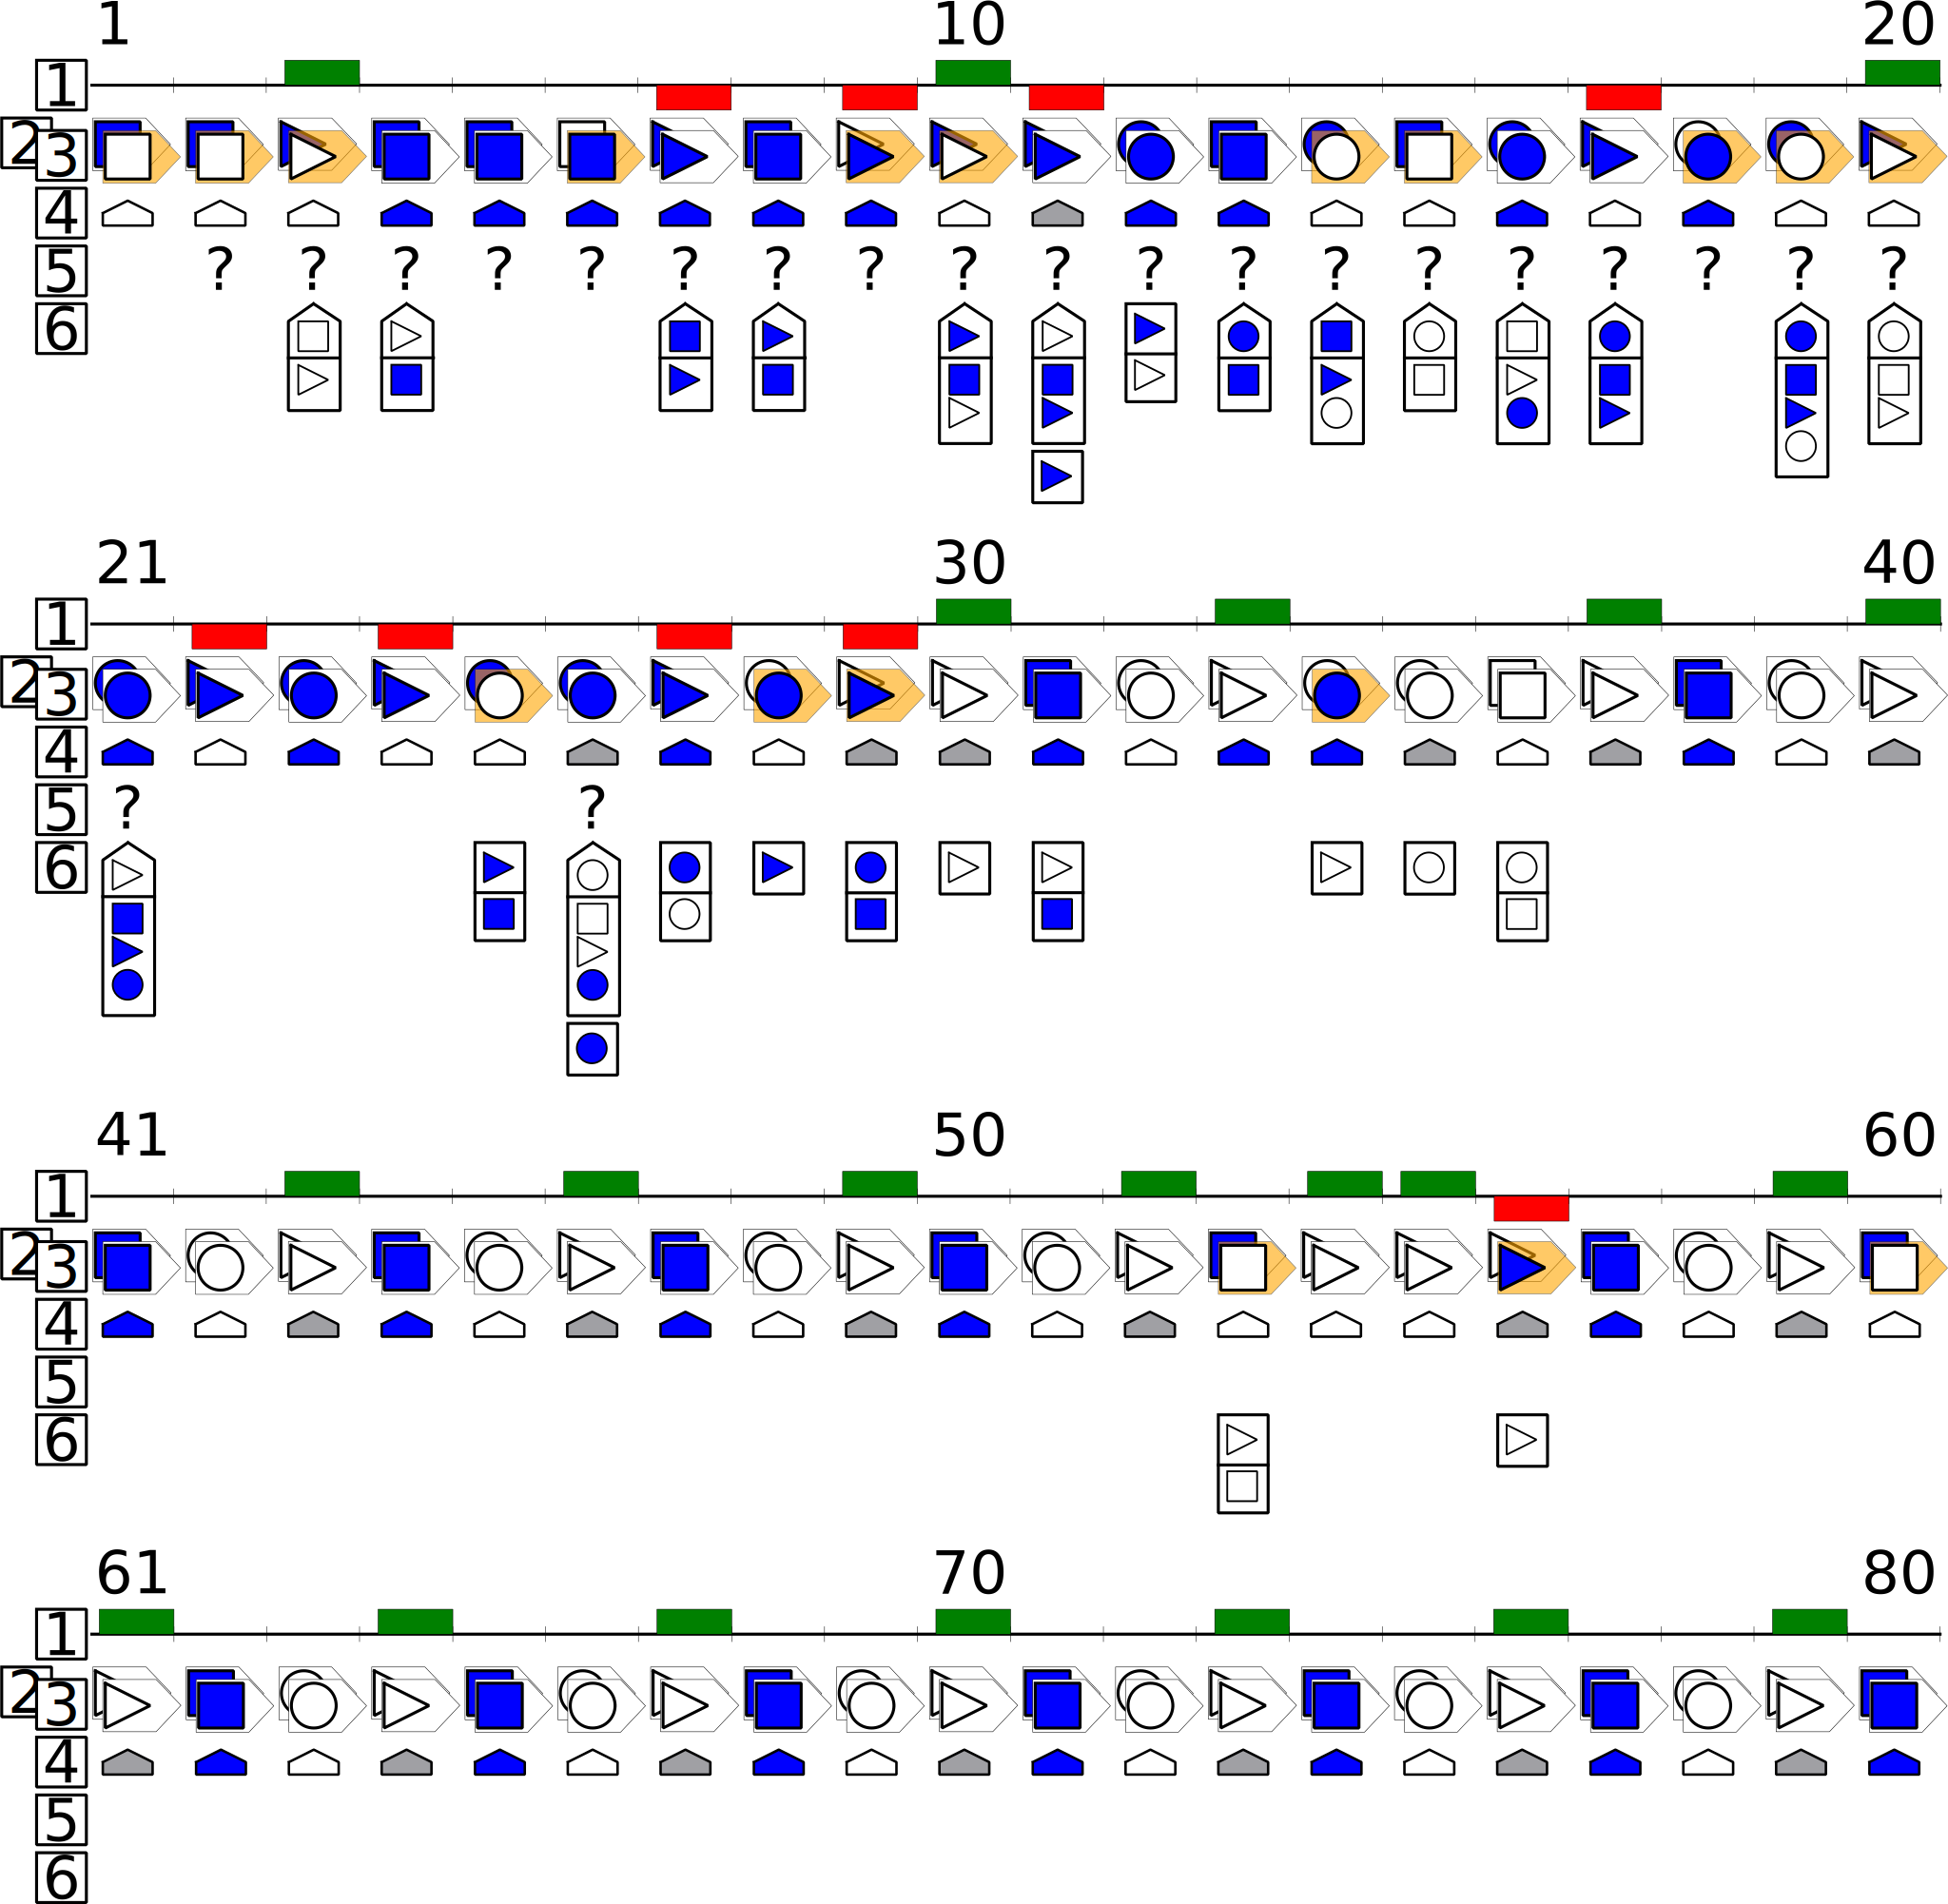
\includegraphics[scale=0.08]{flux_interactions_phenomena_string_problem}
		\caption{80 premières interactions avec l'algorithme d'apprentissage et d'exploitation en simultané.
			Du pas 1 au 21, l'agent possède des tables d'usages vides, il va alors remplir les tables d'usages en testant l'expérience la moins utilisée. Au pas 22, les tables d'usages permettent à l'agent de faire des suppositions et commencer l'exploitation de ses croyances~: il pense que l'interaction \{\triangleBleu\} amène au phénomène \{\triangleBlanc\}. Au pas 25, l'interaction \{\triangleBleu\} met à jour son état de croyance car il a \intended l'interaction \{\rondBleu\} qui est une proposition de l'état de croyance <\triangleBlanc>. Comme l'interaction a échouée, l'état de croyance de l'interaction \{\triangleBleu\} a évolué. Au pas 27, 30 et 35, l'agent apprend que les phénomènes <\rondBleu>, <\triangleBlanc> et <\rondBlanc> sont en réalité des interactions sporadiques. 
			}
		\label{fig:flux_interactions_phenomena_string_problem}
\end{figure}
% A chaque étape
%Pour utiliser les phénomènes, nous avons besoins de faire une distinction entre les interactions persistantes et sporadiques. Une interaction qui peut se répéter indéfiniment représente une interaction persistante. À contrario, une interaction qui ne peut être répétée est appelée interaction sporadique. 
%À travers ces deux concepts, l'agent peut déjà faire la distinction entre une observation et une action sur le monde. % Pourquoi~?


% Def état de croyance, modéliser par pétri, si on a raison alors l'agent doit faire ce 
%À travers le flux d'interactions de la figure \reffig{interactions_flux_string_problem}, on souhaiterai que l'agent arrive à trouver le graphe de Pétri de la figure \reffig{petri_net_string_problem}. Cette représentation permet de visualiser les différentes connexions entre les interactions persistantes et sporadiques.
\begin{figure}
	\centering
	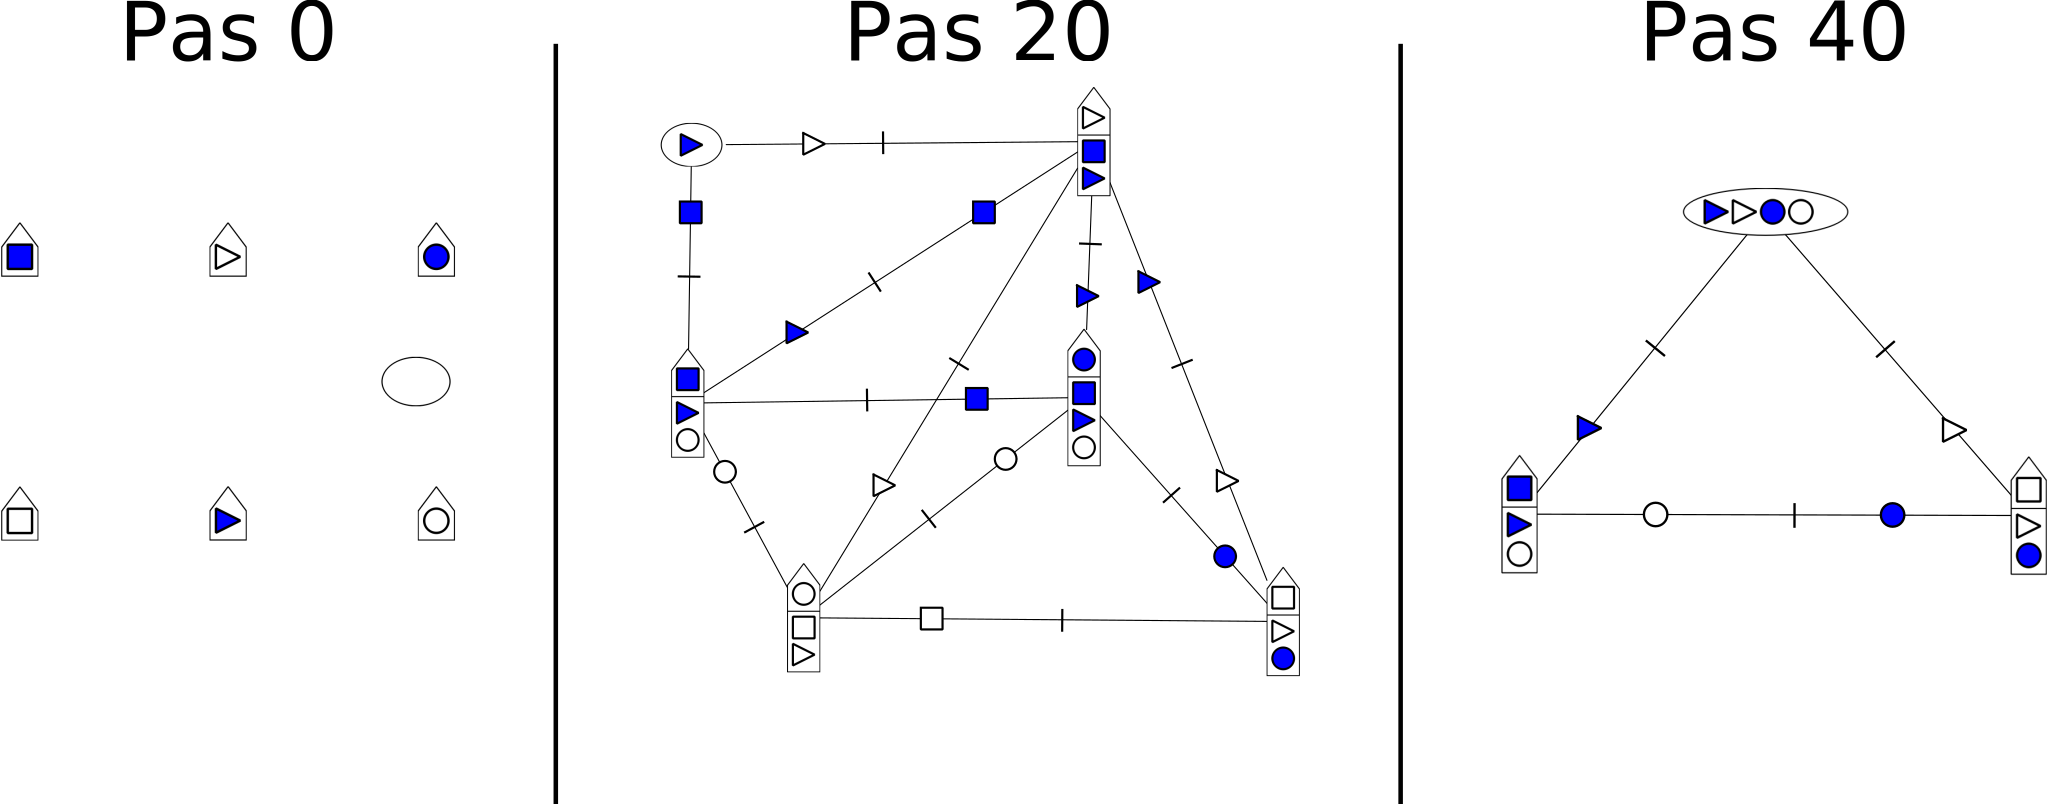
\includegraphics[scale=0.08]{evolve_petri_phenomena_string_problem}
	\caption{Évolution du graphe de Petri.}
	\label{fig:evole_petri_phenomenology_string_problem}
\end{figure}
% Mettre des numero de séquence Attention sac unknown.
%La figure \reffig{petri_net_string_problem} représente l'état de croyance d'un agent. La partie inférieur regroupe les interactions sporadique que l'agent à trouver. On appel cet état de croyance \emph{unknown} car lorsque l'agent est dans cette état il n'a aucune information dans quel état ce trouve l'environnement.
%Il devra alors utilisé l'une des interactions situées dans la partie supérieur du graphe pour déterminer l'état de croyance dans lequel il se trouve. La partie supérieur représente les interactions persistantes.
%L'interaction \num{1} est l'interaction persistente. La partie inférieur du bloc représente les interactions qui pourront être réalisées lorsque l'agent se trouve dans cette état de croyance. 

% Et le trait de séparations permettent d'arriver à l'arriver
%Les arcs représentes les liaisons entre les différents état de croyance. Les interactions situé près d'un état de croyance permettent de passer vers l'autre état de croyance. Par exemple~: lorsque l'agent est dans l'état de croyance \carreBlanc, il pourra passer vers l'état de croyance unknown via l'interaction \triangleBlanc et vers l'état de croyance \carreBleu via l'interaction \rondBleu. 
%L'interaction \rondBleu est une interaction sporadique, mais celle-ci possède une croyance~: il est toujours possible de réaliser l'interaction \carreBlanc après avoir été exécutée. Cette croyance permet d'omettre de réaliser l'interaction \carreBlanc et de choisir de faire directement l'interaction \triangleBlanc après avoir réaliser l'interaction \rondBleu. 

% Il ne cnostruit pas le graphe mais les tables d'usage.
%Pour permettre une tel interprétation par l'algorithme, nous mettons en place une structure appelé tables d'usage.



%\section{Expérience}
%\subsection{Apprentissage}
%Pour mettre en évidence l'utilité de la tables d'usage, un premier algorithme à été développer permettant dans un premier temps de remplir la tables d'usages, sans prendre en considération la valence des interactions puis dans un deuxième temps, exploiter les tables d'usages pour maximiser la motivation interactionnelle comme d'écrit par l'algorithme \refalg{minimum_algorithm_intended} et \refalg{minimum_algorithm_enacted}. Ces deux algorithmes sont la base de la décision. 
%

%La boucle de décision commence par l'algorithme \refalg{minimum_algorithm_intended} puis finis par \refalg{minimum_algorithm_enacted}. Cet algorithme permet de mettre à jour l'humeur de l'agent en fonction de l'interaction enacted. 
%
%La trace de la figure \reffig{minimum_algorithm_flux} montre la réalisation des algorithmes dans l'environnement. L'agent arrive a trouvé les régularités immédiates et séquentielles de l'environnement. Il construit également le graphe de Pétri, mais des lacunes apparaissent. Cela n'est pas un problème car les croyances de l'agent lui permettent de satisfaire sa motivation interactionnelle. 
%\subsection{Apprentissage et exploitation en simultané}
%Grâce à la structure des usages tables, un agent peut réussir à réaliser la trace de la figure \reffig{whole_interactions_flux_string_problem}. Ce flux d'interaction montre l'apprentissage que l'agent met en place avec l'évolution de ces croyances. 
%
%\begin{figure}
%	\centering
%	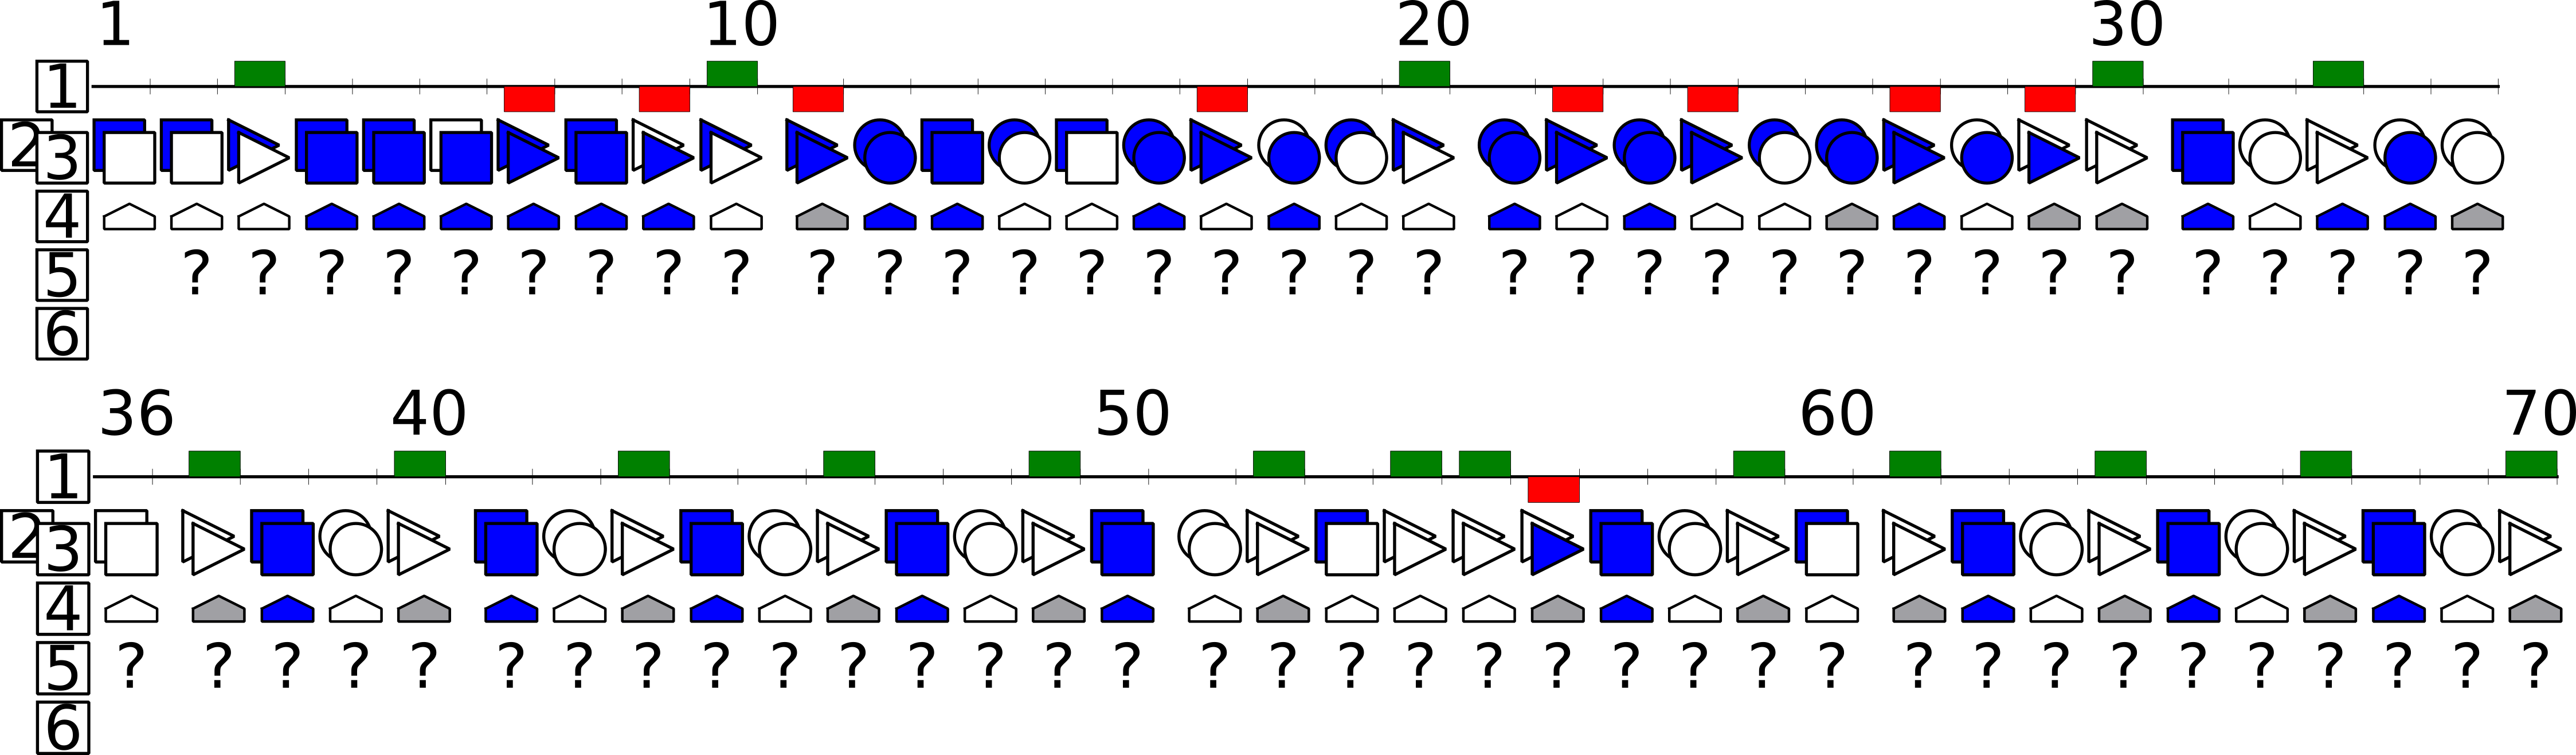
\includegraphics[scale=0.13]{whole_interactions_flux_string_problem}
%	\caption{70 premières interactions dans un environnement réaliser par un agent implémentant l'algorithme de la meilleur interaction}
%	\label{fig:whole_interactions_flux_string_problem}
%\end{figure}
%% Explication du graphe
%La ligne \num{1} de la figure, représente la valence de l'interaction. En vert, la valence est positive, en rouge négative et nulle lorsque il n'y a que le trait. L'interaction intended est sur la ligne \num[2] et l'interaction enacted sur la \num{3}. La ligne \num[4] représente la couleur de l'état de croyance. L'humeur de l'agent est sur la ligne \num[5]. Le point d'interrogation représente une humeur curieux, rien pour la sélection de la meilleur interaction possible dans le \emph{contexte} courant. La ligne \num{[6]} est une représentation de la création et modification d'une interaction persistante.
%
%
%% Explication du point de vue de l'agent
%Les interactions sont pré-supposées persistante lors de l'initialisation de l'agent. De l'étape 1 à 40, l'agent teste les différentes interactions sans savoir vraiment ce qui ce passe. Il pense que chaque interaction est une interaction persistante et va essayer de voir si c'est vraiment le cas. Les différentes tables d'usages se mettent à jour afin de régler les problèmes directement accessible quant aux croyances créées lors de l'initialisation. Il met à jour les tables d'usages lui permettant par la suite de satisfaire ça motivation interactionnelle. Tant que l'agent n'arrive pas à trouver un graphe de Pétri lui permettant d'\emph{avancer} celui-ci va tester les différentes interactions afin de trouver des arrêtes lui permettant de passer d'une interaction non.


%\section{Environnement de travail}
\newpage
\section{Un environnement pour le développement et l'étude d'agents développementaux}

En parallèle de mes travaux sur la construction des connaissances par les agents, j'ai développé un environnement de travail destiné à accompagner ces travaux.
Cet environnement, dont une interface est présentée figure~\reffig{screenshot_prog_principal} permet de déployer différents types d'agents dans différents environnements, et de visualiser différents éléments au fil de l'exécution.
Parmi ces éléments, on retrouve~: les tables d'usage construites par l'agent, le graphe de Pétri déduit des tables d'usages, et enfin, les traces d'interaction produites par l'agent (interactions, évolution de la satisfaction, etc.).

Cet environnement, dont les fonctionnalités ont évoluées tout au long du stage, permet donc de supporter activement le développement et le débugage d'agents développementaux. Cela en permettant au concepteur d'exécuter différentes stratégies et de visualiser en temps réel les conséquences de ces stratégies sur le comportement des agents.
De plus, l'outil permet de produire des visualisations graphiques explicites qui peuvent être exportées afin d'expliquer et d'illustrer les concepts mis en œuvre dans les agents.
À titre d'exemple, l'ensemble des traces présentées dans ce rapport a été généré depuis l'environnement. 

J'ai développé cet environnement dans l'optique de faciliter son utilisation et son extension par d'autres. % Langage, site web.
%Le logiciel développé durant le stage a été réalisé dans l'optique d'être réutilisé par la suite.
Il est composé de 4 librairies ainsi que d'un programme principal qui les lient entre elles.
 
La première librairie donne l'implémentation des agents, des mécanismes d'apprentissage et d'exploitation des interactions.
C'est cette librairie qu'il faut enrichir si l'on souhaite étendre les mécanismes d'apprentissage ou expérimenter de nouvelles stratégies d'exploitation des interactions. 

La seconde librairie permet de réaliser une simulation d'un agent dans un environnement donné.

La troisième librairie contient les outils requis pour la construction des visualisations graphiques des interactions et des tables d'usage.
 
La dernière librairie permet de lier l'environnement à un serveur de type KTBS\footnote{KTBS~: Kernel for Trace Base System dont les concepts sont disponibles à l'adresse~:
  \url{https~://kernel-for-trace-based-systems.readthedocs.org/en/latest/concepts/overview.html}}.
Les KTBS sont des outils dédiés au stockage de traces.
Cette librairie permet donc d'enregistrer toutes les traces d'exécution d'une expérimentation dans un serveur dédié pour pouvoir, par exemple, les réutiliser de façon asynchrone sans avoir à ré-exécuter les agents.
Actuellement, cette fonctionnalité de réutilisation n'est pas implémentée, mais lorsqu'elle le sera, cela permettra aux utilisateurs de pouvoir visualiser et comparer des résultats d'expérimentations à tout moment sans avoir à reconfigurer l'ensemble de l'environnement pour chaque expérimentation. 

Cet environnement a été intégralement développé en C++ et est disponible sous licence GPL à l'adresse suivante~: \url{https~://gforge.liris.cnrs.fr/anonscm/git/devlearnremiflo/devlearnremiflo.git}

%Le programme principal représenté par la figure \reffig{screenshot_prog_principal} montre un agent utilisant l'algorithme d'apprentissage et d'exploitation simultané dans le \emph{string problem} au centre.

%La partie inférieure du programme montre une partie de la librairie graphique d'interaction.

\begin{landscape}
	\begin{figure}
		\centering
		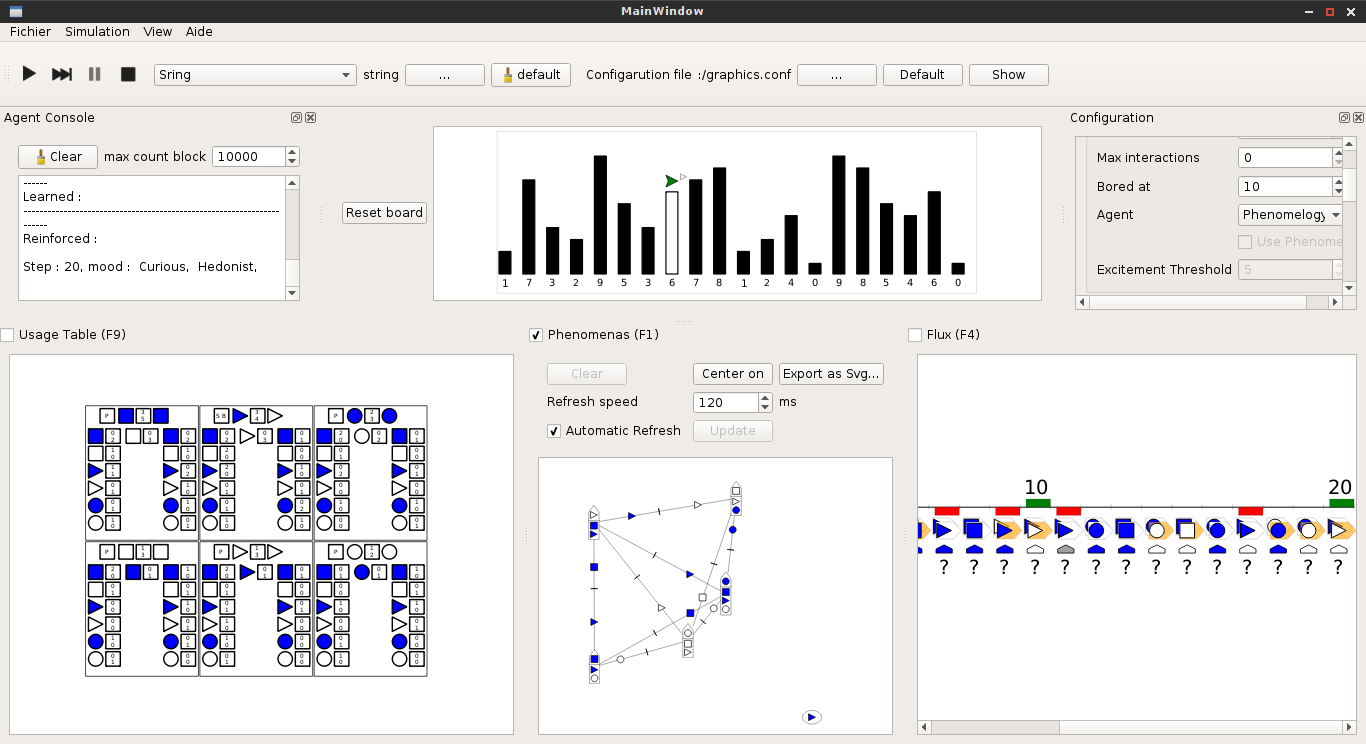
\includegraphics[scale=0.4]{screenshot_prog_principal}
		\caption[Exemple d'interface de l'environnement de développement]{Dans cet exemple, un agent évolue dans le \emph{string problem}. La partie inférieure propose plusieurs types de visualisation. Dans la partie supérieur droite se trouve la configuration de la simulation. L'affichage des logs de l'agent, apparaissent eux à gauche. On peut y voir les interactions activées, proposées, \intended, \enacted, apprises et renforcées et les humeurs de l'agent. Dans le menu, il est possible de sélectionner l'environnement avec son fichier de configuration. À droite, le fichier de configuration du graphisme. 
                } % TODO~: adapter la légende.
                
		\label{fig:screenshot_prog_principal}
	\end{figure}
\end{landscape}

\section{Conclusion}
L'approche développementale permet de construire un agent agnostique qui ne possède pas d'information sur son environnement. À travers ses interactions, l'agent va apprendre à interagir avec le monde pour satisfaire sa motivation interactionnelle. Ce rapport montre comment, à partir d'un flux d'interactions, un agent peut construire des connaissances liées aux régularités observées. L'agent représente des \og~choses~\fg à travers ses interactions sans pour autant avoir un accès direct aux \og~choses~\fg.
Cette représentation soulève et laisse ouvertes de nombreuses questions comme: comment représenter des phénomènes avec des interactions composites, est-ce que les tables d'usage associées aux interactions composites donneront à l'agent la possibilité d'appréhender les environnements spatiaux impliquant la présence de plusieurs phénomènes à des endroits différents~? 

Du côté de la motivation décisionnelle, nous avons détaillé deux algorithmes mettant en œuvre des formes d'excitation~: la curiosité et l'hédonisme. D'autres motivations existent mais n'ont pas été implémentées~:
\begin{itemize}
	\item la simulation interne d'une interaction composite basée sur les connaissances de son environnement dans la perspective de trouver, voire de créer, une interaction plus satisfaisante~;
	\item la possibilité de se concentrer sur un objectif (représenté par une interaction primitive ou composite) pour déterminer s'il est atteignable ou non.
\end{itemize}
% On partie de ce constat... pour tenter de résoudre ce problème, on a fais ça parrapport à l'état de lart, du coup on est arrivé à ca. En continuant dans cette direction, nous souhaitons que l'agent développe une manière de représenter un environnement spatial. On pourra alors se pencher sur une structure permettant à l'agent d'apprehender l'espace à travers ses interactions.
%L'implémentation d'un agent agnostique utilisant les préceptes de l'apprentissage développemental n'est pas chose facile. L'avancée que j'ai réalisé me semble insignifiante et pourtant ce n'est pas chose facile que d'aller plus loin. L'implémentation de nouveaux algorithmes d'apprentissage et d'exploitation d'interactions 

\bibliographystyle{alpha}
\bibliography{bibliographie}

\end{document}
